%%%%%%%%%%%%%%%%%%%%%%%%%%%%%%%%%%%%%%%%%%%%%%%%%%%%%%%%%%%%%
% This document can be formatted only with pdflatex.
%%%%%%%%%%%%%%%%%%%%%%%%%%%%%%%%%%%%%%%%%%%%%%%%%%%%%%%%%%%%%

% TODO use the T-CREST template here

\documentclass[11pt,twoside,a4paper]{article}
\usepackage[margin=1.1in]{geometry}

\usepackage{hyperref}
\usepackage[T1]{fontenc}
\usepackage{ae}
\usepackage[pdftex]{graphicx}
\usepackage[english]{babel}
\usepackage{latexsym,epsf,epsfig}
\usepackage{rotating,amsmath,amsfonts,amssymb,subfigure}
\usepackage{amsthm}

\usepackage{times}
\usepackage{listings}
\usepackage{longtable}
\usepackage{datetime}
\usepackage{verbatim}
\usepackage{tabularx}
\usepackage{multirow}
\usepackage{array}

\usepackage{booktabs}
\usepackage{dcolumn}

\usepackage{pslatex} % -- times instead of computer modern
\usepackage{url}
\usepackage{graphicx}
\usepackage{textcomp}
\usepackage{xspace}
\usepackage[usenames,dvipsnames]{xcolor}
\usepackage{colortbl}
\usepackage{multicol}

\usepackage{bytefield}

% TODO move the ISA related stuff into the isa.tex file

% long immediate in second slot
\newcommand{\lconst}{\texttt{const}_{32}}
% short immediate in ALU instruction
\newcommand{\sconst}{\texttt{Constant}_{12}}
% constant in Rs2 field
\newcommand{\rconst}{\texttt{Constant}_{5}}


\newcommand{\cc}[1]{\multicolumn{1}{c}{#1}}
\newcolumntype{d}[1]{D{.}{.}{#1}}
\newcommand{\code}[1]{{\texttt{#1}}}
\newcommand{\codefoot}[1]{{\texttt{#1}}}
\newcommand{\eg}{\emph{e.g.}}
\newcommand{\ie}{\emph{i.e.}}

\usepackage{listings}
\lstset{language=C,basicstyle=\footnotesize,captionpos=b}
%% \renewcommand{\lstlistingname}{\footnotesize Listing}

\newtheorem{lemma}{Lemma}
\newtheorem{theorem}{Theorem}
\newtheorem{criterion}{Criterion}
\newtheorem{definition}{Definition}

\newcommand{\XOR}{\textasciicircum\xspace}
\newcommand{\OR}{\textbar\xspace}
\newcommand{\AND}{\&\xspace}
\newcommand{\NOT}{\texttildelow}
\newcommand{\shl}{\textless$\!$\textless\xspace}
\newcommand{\shr}{\textgreater$\!$\textgreater$\!$\textgreater\xspace}
\newcommand{\ashr}{\textgreater$\!$\textgreater\xspace}

%
% allow click-able links
%
\usepackage[open]{bookmark}
\usepackage[all]{hypcap}

% \pdfcatalog{
%  /UseNone
% }

\title{The Patmos Tool Chain Manual}

\begin{document}

%\firstpage
\maketitle

\newpage
\tableofcontents

\newpage

\cleardoublepage
%\pagenumbering{arabic}


% % % % % % % % % % % % % % % % % % % % % % % % % % % % % % % % % % % % % % % % 

% TODO needs cleanup, currently not fully up-to-date.
% % % % % % % % % % % % % % % % % % % % % % % % % % % % % % % % % % % % % % % % 
\chapter{The Patmos Compiler}
\label{sec:the_patmos_compiler}

The principal components of the tool chain currently are:
(1) the C frontend \texttt{Clang},\footnote{\url{http://clang.llvm.org/}} (2)
the LLVM optimisers, (3) an LLVM-based code generator and LLVM-based utilities
for the Patmos processor, (4) the \texttt{gold} linker of the binutils project,%
\footnote{\url{http://sourceware.org/binutils/}} (5) the \texttt{newlib} C
library,\footnote{\url{http://sourceware.org/newlib/}} and (6) the compiler
support library \texttt{compiler-rt}.%
\footnote{\url{http://compiler-rt.llvm.org/}}

\section{Tool Chain Overview}
\label{sec:toolchain_overview}

Figure~\ref{fig:framework} depicts a typical compilation flow of the Patmos
tool chain. First, the C source code of a user-supplied application is
translated to LLVM bitcode using the \texttt{clang} frontend. Next, the
generated bitcode files are linked with the system libraries (e.g., the 
\texttt{newlib} C library) using the LLVM tool \texttt{llvm-ld}. This results in
one combined bitcode file, which contains all user- and system code of the
application. The \emph{linked} application can then be optimised using the
high-level optimisations of LLVM, which are readily available through
\texttt{llvm-ld}. In the following step the linked and optimised bitcode is
translated to machine code using the Patmos code generator and the LLVM tool
\texttt{llc}. This results in a relocatable ELF binary, which already contains
the entire machine code of the application and thus is, in principle, ready to
be executed. The final step of the tool chain performs the final code and data
layout of the application using the \texttt{gold} linker and an optional,
user-supplied linker script. Note that no new code is added at this step since
all libraries were already linked at the bitcode-level beforehand. This
compilation flow was specifically designed to facilitate the development of
future WCET-driven compilation techniques within the T-CREST project. Since all
the application code is linked into a single bitcode file, the LLVM optimisers
and the Patmos code generator have a complete view of all the application code
needed to optimise the WCET.

\begin{figure}[t]
  \centering
  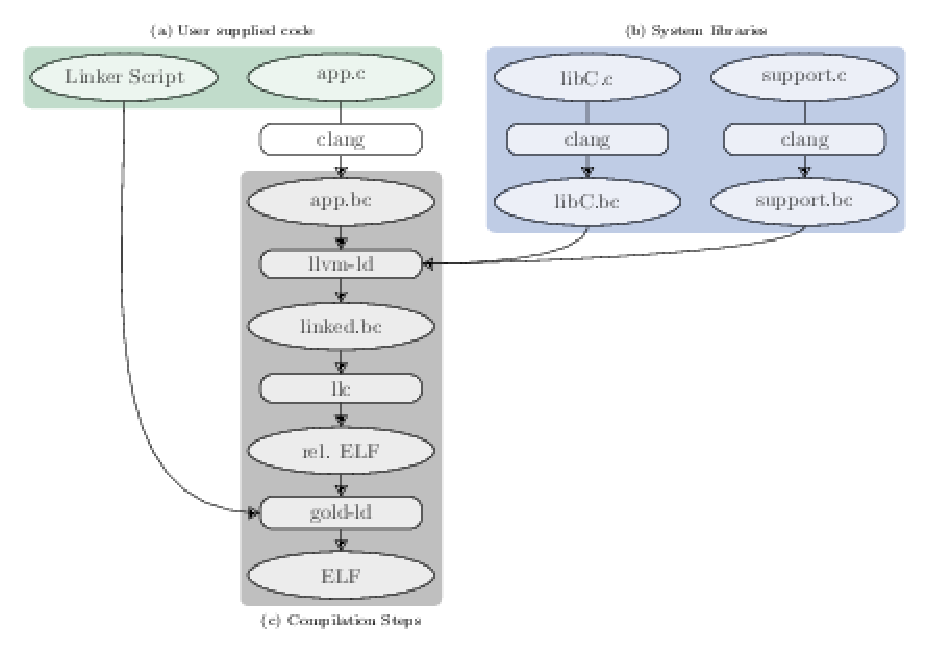
\includegraphics{fig/framework}

  \caption{Compilation flow of the Patmos tool chain.}
  \label{fig:framework}
\end{figure}

The following section describes each of these components in more detail.

% ------------------------------------------------------------------------------
\section{Principal Components}

% TODO:
%   clang, llvm-ld, llc, gold, newlib, compiler-rt
%   mention LLVM generated assembler and disassembler
%   simulator?

\begin{description}
\item[clang] \hfill\\
  \texttt{clang} is the C frontend that translates source code files written in C
  to the LLVM intermediate representation (aka \emph{bitcode}). The bitcode
  is the representation the LLVM analyses and optimisations work upon.
  \texttt{clang} also acts as a driver that invokes the tools involved with the
  options specific for targeting Patmos.

  \begin{tabular}{ll}
  Input:  & \texttt{.c} source code file \\
  Output: & \texttt{.bc} bitcode object file
  \end{tabular}

\item[llvm-ld] \hfill\\
  \texttt{llvm-ld} links bitcode files and static libraries of bitcode files
  together into a bitcode file containing the bitcode from the input files
  and the required symbol definitions from the libraries.

  \begin{tabular}{ll}
  Input:  & \texttt{.bc} bitcode object files [, \texttt{lib*.a} bitcode
            libraries ]\\
  Output: & \texttt{.bc} linked bitcode object file
  \end{tabular}

\item[llc] \hfill\\
  \texttt{llc} constitutes the backend translating a bitcode file into either
  assembly or binary machine code for the Patmos ISA.
  The binary output format is relocatable ELF.

  \begin{tabular}{ll}
  Input:  & \texttt{.bc} bitcode object file \\
  Output: & \texttt{.s} Patmos assembly \\
          & or \texttt{.o} Patmos relocatable ELF
  \end{tabular}

\item[gold] \hfill\\
  \texttt{gold} is an ELF linker.
  In our tool chain it is adopted to perform relocations.

  \begin{tabular}{ll}
  Input:  & \texttt{.o} Patmos relocatable ELF \\
  Output: & \texttt{.o} Patmos final ELF
  \end{tabular}

\item[C Library] \hfill\\
  We adopted \texttt{newlib}, a
  standard ANSI C library following the C90 and C99 
  standards~\cite{ISO:9899:1990,ISO:9899:1999}, for Patmos. In the Patmos 
  compilation flow the entire \texttt{newlib} C library is translated to LLVM 
  bitcode and linked as such with the application program \emph{before} code 
  generation. This is an important precondition for WCET-driven compilation as 
  envisioned in the T-CREST project, as it provides the compiler with a complete 
  view of \emph{all} code belonging to an application.

\item[Support Library] \hfill\\
  The LLVM compiler requires a support library, which provides for instance 
  emulation functions for floating-point operations. LLVM's 
  \texttt{compiler-rt} support
  library has been adopted for Patmos and is, similar to the C library, compiled 
  to LLVM bitcode and linked with the application program if needed.
\end{description}



% TODO organize the structure properly:
% - Make a report out of this, introduce chapters
% - Use the following structure (maybe):
%   - Platform Overview
%   - Patmos Core
%	- Architecture
%	- Simulator
%	- Synthesizing, booting
%   - Compiler Tool Chain
%	- Overview, Components
%	- Clang Frontend
%	- LLVM Backend
%	- ELF Binary
%   - WCET Analysis and WCET integration
%	- aiT
%	- Platin
%   - Installation and Usage
%	- Build script
%	- Compiler Usage
%   - Appendix
%	- ISA Reference
%	- Examples
%
% How do we organize this: We have 
%   - Components: Patmos Core, Simulator, Compiler Tool Chain, WCET Analysis, Platin, NoC, RTEMS, ...
%   - Common Structure: Overview, Description, Full Reference/Specs, Installation, Tool Usage, Examples, ...
% Do we top-level-organize by component or by structure??? Better approach is probably by Structure, 
% since some components share same specs, same build system .. -> Have main chapters for
%   - Platform Overview (big picture, all the buzzwords)
%   - More In-depth description of various components (still high-level (no technical stuff), but with all the nasty details, results ..; similar to paper style)
%   - Specifications (Common: ISA, ABI, ELF format, asm format, IO-ports, Target Triples, ..; plus component-specific: Clang Frontend, Platin
%     PML, newlib, ..)
%   - Installation and Usage: Sections for build.sh, platin, aiT, NoC?, RTEMS, Synthesizing and booting Patmos, ..
%     This should not include stuff that is already in any README.patmos file (configure-strings, list of options, ..) if possible!
%     Just the big picture, stuff that is too long for the README; the most important stuff can be repeated, plus a reference to the README.
%   - (Bigger) Usage Examples
%	- Hello world, ...
%	- Reference and describe demos in patmos-misc/demo/
%
% To conclude
% - create chapters, clean up main structure
% - move (inline) asm stuff from patmos_tr here
% - remove stuff from here that is already in READMEs and should not be repeated here (manual building without build.sh, ..)
% - move patmos-misc/doc/*.txt stuff into content, convert to tex
% - use the T-CREST template style
% - Somehow copy the ISA part from TR to here, fix formatting.
% - clean up this whole mess, make sure everything is consistent/up-to-date


% TODO this is (partially) redundant with the README.patmos files. We should put
% compile instructions only in README.patmos files and only describe the build.sh 
% script and some top-level build instructions here.

\section{Installation and Usage of the Compiler}
\label{sec:using_the_compiler}

This section gives a guide for building and installing the Patmos
tool chain and describes how to use it to compile applications for Patmos. 

% ------------------------------------------------------------------------------
\subsection{Prerequisites}

The Patmos compiler tool chain is developed for the Linux platform. 
In order to build all tools, the following programs and libraries are required:

\begin{description}
\item[cmake, make] \hfill\\
The CMake (at least version 2.8) and \texttt{make} build systems are required to build the
various components of the tool chain, such as the \texttt{clang} compiler or the \texttt{compiler-rt} system library.
\medskip

\item[gcc, g++] \hfill\\
A C and C++ compiler such as GCC is required to build \texttt{clang}, \texttt{llvm}
and \texttt{gold}. It is also possible to use a separate \texttt{clang} installation as 
an alternative to GCC. Compiling with \texttt{clang} will result in shorter compile
times, however, if the compiled application should be debugged with \texttt{gdb}, it is
recommended to use \texttt{gcc} and \texttt{g++}.
\medskip

\item[flex, bison, texinfo] \hfill\\
These tools are required to build tools such as gold successfully.
\medskip

\item[libelf] \hfill\\
The tools in the Patmos tool chain require the development headers of \texttt{libelf},
as this library is used to read and write ELF files.
\medskip

\item[boost] \hfill\\
The simulator requires the program-options library from the \texttt{boost} C++ library
(at least version 1.46).
\medskip

\item[git] \hfill\\
The version control system \texttt{git} is required 
to download the latest development versions of the tools. 
\end{description}

On current Debian based Linux distributions, the following command can be used to install
all the required packages:

\begin{verbatim}
sudo apt-get install git cmake make g++ texinfo flex bison \
  libelf-dev graphviz libboost-dev libboost-program-options-dev
\end{verbatim}

% ------------------------------------------------------------------------------
\subsection{Retrieving and Building the Source Code}

We provide a build script that retrieves, configures and builds all
the required packages automatically (cf. Section~\ref{sec:buildscript}).
Alternatively, the various tool chain source repositories can be acquired individually from 
the \texttt{t-crest} organisation at \texttt{github.com}.\footnote{\url{http://github.com/t-crest/}}, as
described in Section~\ref{sec:manual_build}. 

We created a tag called \texttt{release\_m12} in all tool chain related source repositories mentioned in this report
that marks the current stable release version of the various tools at the time of writing.
To build the released compiler version instead of the latest development version, execute the following command
in all of the source repositories after they have been checked out, and then rerun the build commands.

\begin{verbatim}
git checkout release_m12
\end{verbatim}

Alternatively, \texttt{github.com} provides a link in all of the source repositories to download the source code for that tag as 
zip files.


%\subsubsection{Default Directory Structure}

For the following build instructions we use directory structure presented in Table~\ref{tab:directories}. 
We use \texttt{\textasciitilde/tcrest/} as root directory and \texttt{\textasciitilde/tcrest/local/}
as installation directory in this document. However, the root directory and the installation directory
can be chosen arbitrarily.

\newcommand{\rootdir}[1]{\texttt{\textasciitilde/tcrest/#1}}
% Uuugly!
\newcommand{\myspace}{2mm}
\begin{table}
\centering
\begin{tabularx}{\textwidth}{lX}
Directory & Description \\ \hline
\rootdir{} & Base directory (\texttt{ROOT\_DIR}) \\ [\myspace]
\rootdir{patmos} &  Processor source repository \\ [\myspace]
\rootdir{patmos/simulator} & Simulator sources \\ [\myspace]
\rootdir{patmos/simulator/build/} & Simulator build directory \\ [\myspace]
\rootdir{compiler-rt/} & System library source repository  \\ [\myspace]
\rootdir{compiler-rt/build/} & System library build directory \\ [\myspace]
\rootdir{gold/} & ELF linker and \texttt{binutils} sources \\ [\myspace] 
\rootdir{gold/build/} & Linker and \texttt{binutils} build directory \\ [\myspace]
\rootdir{llvm/} & LLVM source repository \\ [\myspace] 
\rootdir{llvm/tools/clang} & Clang source repository. Must always be a 
			    \texttt{tools/clang} subdirectory of LLVM \\ [\myspace]
\rootdir{llvm/build/} & Build directory for LLVM and clang \\ [\myspace] 
\rootdir{local/} & Install base directory (\texttt{INSTALL\_DIR}) \\ [\myspace]
\rootdir{local/bin/} & Install directory for tool chain binaries. 
                       All binaries in this directory are prefixed 
		       with \texttt{patmos-} by the build script \\ [\myspace]
\rootdir{local/lib/} & Install directory for tool chain libraries \\ [\myspace] 
\rootdir{local/patmos-unknown-unknown-elf/} & Install directory for Patmos 
                                       libraries and headers \\ [\myspace]
\rootdir{misc/} & Support files (e.g., build script, config files) \\ [\myspace]
\rootdir{newlib/} & Sources of standard C library for Patmos \\ [\myspace]
\rootdir{newlib/build/} & Standard library build directory 
\end{tabularx}
\caption{Default directory structure of the tool chain}
\label{tab:directories}
\end{table}

\subsubsection{Building the Tool Chain Using the Build Script}
\label{sec:buildscript}

After installing the prerequisites, download or check out the build script 
from the \texttt{patmos-misc} repository on \texttt{github.com}:

\begin{verbatim}
git clone https://github.com/t-crest/patmos-misc.git misc
\end{verbatim}

To configure the build script, place a configuration file called \texttt{build.cfg}
into the same directory as the \texttt{build.sh} script. 
In this configuration file, set the \texttt{ROOT\_DIR} variable to the directory which should contain all
the repository checkouts and build directories (e.g., \texttt{ROOT\_DIR=\textasciitilde/tcrest/}).

\begin{verbatim}
cd misc
cp build.cfg.dist build.cfg
# edit build.cfg, set ROOT_DIR and INSTALL_DIR
./build.sh
\end{verbatim}

Executing \texttt{build.sh} checks out any missing repository, configures and then builds
all the required tools and libraries of the tool chain. 
By default, the directory structure created by the build script follows the directory structure presented in Table~\ref{tab:directories}. 
All necessary compiler tools are installed to 
\texttt{INSTALL\_DIR/bin}, while Patmos specific libraries such as \texttt{newlib} and 
\texttt{compiler-rt} are installed under \texttt{INSTALL\_DIR/patmos-unknown-unknown-elf/}.
All executables are prefixed with \texttt{patmos-} to differentiate them from non-Patmos related
installations, e.g., \texttt{clang} will be installed as \texttt{patmos-clang}.


\subsubsection{Building the Tool Chain Manually}
\label{sec:manual_build}

To build all tools and libraries manually, check out and build the following repositories as described below.

\paragraph{The Binary Linker \texttt{gold}} \hfill\\

The following commands build the \texttt{gold} linker for Patmos ELF files.
\begin{verbatim}
git clone https://github.com/t-crest/patmos-gold.git gold
mkdir gold/build
cd gold/build
../configure --program-prefix=patmos- --enable-gold=yes \
    --enable-ld=no --enable-plugins --prefix=~/tcrest/local
make all-gold install-gold
\end{verbatim}

%Optionally, the binutils tools \texttt{ar} and \texttt{nm} for creating and inspecting archives 
%can be built with the command
%\begin{verbatim}
%make all-binutils install-binutils
%\end{verbatim}
%They support the \texttt{LLVMgold.so} plugin provided by LLVM, which enables them to work with archive
%files containing bitcode files.

\paragraph{The Compiler Framework \texttt{llvm} and the C Compiler Tool \texttt{clang}} \hfill\\

The \texttt{patmos-clang} repository must be checked out inside the \texttt{patmos-llvm} repository checkout as
\texttt{tools/clang} directory (creating a symlink instead is not supported). 
\texttt{Clang} is then built automatically when \texttt{llvm} is built.

\begin{verbatim}
git clone https://github.com/t-crest/patmos-llvm.git llvm
git clone https://github.com/t-crest/patmos-clang.git \
                                         llvm/tools/clang
mkdir llvm/build
cd llvm/build
cmake -DLLVM_TARGETS_TO_BUILD=Patmos \
      -DCMAKE_BUILD_TYPE=Debug \
      -DCMAKE_INSTALL_PREFIX=~/tcrest/local ..
make all install
\end{verbatim}

% Explanation for building LLVMgold.so?

\paragraph{The C Library \texttt{newlib}} \hfill\\

Newlib uses the \texttt{llvm-ar} and \texttt{llvm-ranlib} tools provided by LLVM to build bitcode 
archives, while \texttt{clang} is used to link files. 

\begin{verbatim}
git clone https://github.com/t-crest/patmos-newlib.git newlib
mkdir newlib/build
cd newlib/build
../configure --target=patmos-unknown-unknown-elf \
    AR_FOR_TARGET=~/tcrest/local/bin/llvm-ar \
    RANLIB_FOR_TARGET=~/tcrest/local/bin/llvm-ranlib \
    LD_FOR_TARGET=~/tcrest/local/bin/clang \
    CC_FOR_TARGET=~/tcrest/local/bin/clang \
    CFLAGS_FOR_TARGET="-target patmos-unknown-unknown-elf -O2" \
    --prefix=~/tcrest/local
make all install
\end{verbatim}

Alternatively, the \texttt{ar} and \texttt{ranlib} tools provided by \texttt{patmos-gold} can 
be used to build \texttt{newlib}, provided that LLVM is configured to build the binutils link time optimisation (LTO) plugin that provides
bitcode file support for the binutils tools.
\paragraph{The Support Library \texttt{compiler-rt}} \hfill \\

The following commands build and install the runtime libraries for Patmos.

\begin{verbatim}
git clone https://github.com/t-crest/patmos-compiler-rt.git \
                                                 compiler-rt
mkdir compiler-rt/build
cd compiler-rt/build
cmake -DCMAKE_TOOLCHAIN_FILE=\
        ../cmake/patmos-clang-toolchain.cmake \
      -DCMAKE_PROGRAM_PATH=~/tcrest/local/bin \
      -DCMAKE_INSTALL_PREFIX=~/tcrest/local ..
make all install
\end{verbatim}

The tool chain file \texttt{patmos-clang-toolchain.cmake} sets up the build environment with the tools of the Patmos tool chain 
that are found in the given program path. The compiler-rt libraries are installed
along with the newlib libraries into the default library lookup path
of the Patmos compiler.

\paragraph{The Patmos Simulator \texttt{pasim}} \hfill \\

The simulator for Patmos was part of Deliverable 2.1 and is part of the Patmos processor repository. Compiling the simulator requires an installation of the 
development headers of libboost and libelf. The following commands build and install the simulator.

\begin{verbatim}
git clone https://github.com/t-crest/patmos.git
mkdir patmos/simulator/build
cd patmos/simulator/build
cmake -DCMAKE_INSTALL_PREFIX=~/tcrest/local ..
\end{verbatim}


For more information on building and using the tools, please refer to the \texttt{README.patmos} files 
that are contained in the source repositories.


% ------------------------------------------------------------------------------
\subsection{Running the Compiler}

%In this section we assume that the tools have been compiled and installed with the provided build script,
%i.e., all tools of the Patmos tool chain are prefixed with \texttt{patmos-}.

The compiler is executed by running the compiler driver tool \texttt{patmos-clang}. This invokes the 
necessary tools to compile, assemble and link an application. 

In order to build an application for Patmos, the target platform triple, the output file name and the source files (either C code or bitcode files) 
need to be provided to \texttt{patmos-clang}.

\begin{verbatim}
patmos-clang -target patmos-unknown-unknown-elf -o hello main.c hello.c
\end{verbatim}

This will compile the source files to bitcode files, link in \texttt{newlib} and the system libraries,
and execute \texttt{patmos-gold} to create the final executable application. If the option \texttt{-v} is passed
to \texttt{patmos-clang}, the tools print out all commands that are executed in the background, as well as additional information
about search paths and linked libraries.

After compilation, the application is executed in the simulator by using

\begin{verbatim}
pasim hello
\end{verbatim}

\subsubsection{Driver Options}

The \texttt{patmos-clang} driver can also be used to generate bitcode files, to link bitcode files, or to 
emit assembler code. The driver supports the following modes of operation (for brevity, we omit the
\texttt{-target patmos-unknown-unknown-elf} argument):


\begin{description}
\item[\texttt{patmos-clang -c <inputs>}] \hfill\\
  \begin{tabular}{ll}
  Input:   & \texttt{.c} C source file \\
  Output:  & \texttt{.o} or \texttt{.bc} bitcode files \\
  Actions: & compile each input file to a bitcode file
  \end{tabular}

\item[\texttt{patmos-clang -S <inputs>}] \hfill\\
  \begin{tabular}{ll}
  Input:   & \texttt{.c} C source file \\
  Output:  & \texttt{.s} or \texttt{.ll} human readable bitcode files \\
  Actions: & compile each input file to a human readable bitcode file
  \end{tabular}

\item[\texttt{patmos-clang -emit-llvm <inputs>}] \hfill\\
  \begin{tabular}{ll}
  Input:   & \texttt{.c} C source file, \texttt{.bc} bitcode object file, \texttt{.a} bitcode files archive \\
  Output:  & bitcode file \\
  Actions: & compile to bitcode, link all input files, link with standard libraries and start code \\
\end{tabular}

\item[\texttt{patmos-clang -fpatmos-emit-obj -c <inputs>}] \hfill\\
  \begin{tabular}{ll}
  Input:   & \texttt{.c} C source file \\
  Output:  & \texttt{.o} Patmos relocatable ELF \\
  Actions: & compile each input file to a Patmos relocatable ELF file
  \end{tabular}

\item[\texttt{patmos-clang -fpatmos-emit-obj -S <inputs>}] \hfill\\
  \begin{tabular}{ll}
  Input:   & \texttt{.c} C source file \\
  Output:  & \texttt{.s} Patmos assembly file \\
  Actions: & compile each input file to a Patmos assembly file
  \end{tabular}

\item[\texttt{patmos-clang -fpatmos-emit-obj <inputs>}] \hfill\\
  \begin{tabular}{ll}
  Input:   & \texttt{.c} C source file, \texttt{.bc} bitcode object file, \texttt{.a} bitcode files archive \\
  Output:  & \texttt{.o} Patmos relocatable ELF \\
  Actions: & compile to bitcode, link all input files, link with standard libraries and start code, \\
	   & compile to relocatable ELF
\end{tabular}

\item[\texttt{patmos-clang -fpatmos-emit-asm <inputs>}] \hfill\\
  \begin{tabular}{ll}
  Input:   & \texttt{.c} C source file, \texttt{.bc} bitcode object file, \texttt{.a} bitcode files archive \\
  Output:  & \texttt{.o} Patmos assembly file \\
  Actions: & compile to bitcode, link all input files, link with standard libraries and start code, \\
	   & compile to Patmos assembly
\end{tabular}

\item[\texttt{patmos-clang -o <output> <inputs>}] \hfill\\
  \begin{tabular}{ll}
  Input:   & \texttt{.c} C source file, \texttt{.bc} bitcode object file, \texttt{.a} bitcode files archive \\
  Output:  & Patmos executable ELF \\
  Actions: & compile to bitcode, link with standard libraries and start code, \\
           & compile to relocatable ELF, create Patmos executable ELF
  \end{tabular}

\end{description}

The compiler accepts standard options such as \texttt{-I}, \texttt{-L} and \texttt{-l} to define additional
lookup paths for header files and libraries and to link with (static) libraries.
The behaviour of the linker can be controlled with additional options for \texttt{patmos-clang} 
as shown in Table~\ref{tab:linker_options}.

\begin{table}
\centering
\begin{tabular}{ll}
Option & Description \\ \hline
\texttt{-mfloat-abi=none} & Do not use software floating point libraries when linking \\
\texttt{-nostdlib} & Do not use standard libraries such as \texttt{libc} when linking \\
\texttt{-nolibc} & Do not use \texttt{libc} when linking \\
\texttt{-nodefaultlibs} & Do not use platform system libraries when linking\\
\texttt{-nostartfiles} & Do not use the \texttt{crt0} start file when linking \\
\texttt{-nolibsyms} & Do not use symbol definition files for runtime libraries when\\
                    & linking. Those files prevent the linker from removing any \\
		    & functions for which calls might be generated by the compiler \\
		    & backend, such as software division or \texttt{memcpy} \\
\texttt{-fpatmos-link-object} & Link as object, i.e., do not link in any libraries or start code 
\end{tabular}
\caption{Options for \texttt{patmos-clang} that control the default behaviour of the linker}
\label{tab:linker_options}
\end{table}

\subsubsection{Libraries}

The Patmos tool chain supports static libraries. Libraries are archives that contain
bitcode files. The archives are created by using either the \texttt{ar}
tool provided by the host system or by using \texttt{patmos-ar} from the \texttt{patmos-gold} binutils. The tool
\texttt{patmos-llvm-nm} can be used to inspect the content of the archive.

\begin{verbatim}
ar q libtest.a *.bc
# show the contents of libtest.a
patmos-llvm-nm libtest.a
# compile and link with the created library
patmos-clang -target patmos-unknown-unknown-elf -o app main.c -ltest
\end{verbatim}


% Anything else? -Wl, .. 




\section*{Appendix}

\appendix

% TODO Ok, now this looks properly horrible without the two-column formatting. Needs cleanup
% and must be put into a chapter, otherwise it messes up the TOC.
% TODO we also need a good way to keep this in sync with the TR.. maybe split the TR into files 
% or export the TR as PDF and only link in the PDF here?
%\section{The Architecture of Patmos}
\label{sec:arch}

\subsection{Pipeline}

Figure~\ref{fig:pipeline} shows an overview of Patmos' pipeline. The pipeline
consist of 5 stages: (1) instruction fetch (\texttt{IF}), (2) decode and
register read (\texttt{DR}), (3) execute (\texttt{EX}), (4) memory access, and (5) register write  back (\texttt{WB}).

Some instructions define additional pipeline stages. Multiplication instructions
are executed, starting from the \texttt{EX} stage, in a parallel pipeline with
fixed-length (see the instruction definition). The respective stages are
referred to by \texttt{EX$_1$}, \dots, \texttt{EX$_n$}.

\begin{figure*}
    \centering
    \includegraphics[scale=0.6]{fig/pipeline}
    \caption{Pipeline of Patmos with fetch, decode, execute, memory, and write back stages.}\label{fig:pipeline}
\end{figure*}


\subsection{Register Files}

The register files available in Patmos are depicted by
Figure~\ref{fig:registers}. In short, Patmos offers:
\begin{itemize}
  \item [-] 32, 32-bit general-purpose registers (\texttt{R}) : \verb!r0, ..., r31! \\
            \verb!r0! is read-only, set to zero (\texttt{0}).
  \item [-] 16, 32-bit special-purpose registers (\texttt{S}): \verb!s0, ..., s15!
  \item [-] 8, single-bit predicate registers (\texttt{P}): \verb!p0, ..., p7!, \\
            \verb!p0! is read-only, set to \texttt{true} (\texttt{1}).
\end{itemize}

All register reads to the \texttt{R}, \texttt{S}, and \texttt{P} register files
are executed in the \texttt{DR} stage. Register writes to \texttt{R} are
performed in the \texttt{MW} stage, while \texttt{S} and \texttt{P} are written
immediately in the \texttt{EX} stage.

Concurrently writing and reading the same register in the same cycle will, for
the read, yield the value that is about to be written.

When writing concurrently to the same register, i.e., the two instructions of
the current bundle have the same destination register, the value of the second
slot is taken, unless the predicate of that instruction evaluates to
\texttt{false} (0).

The predicate registers are usually encoded as $4$-bit operands, where the most
significant bit indicates that the value read from the register file should be
inverted before it is used. For operands that are written, this additional bit
is omitted.

The special-purpose registers of \texttt{S} allow access to some dedicated
registers:
\begin{itemize}
  \item [-] The lower $8$ bits of \texttt{s0} can be used to save/restore
            \emph{all} predicate registers at once. The other bits of that
            register are currently reserved, but not used.
  \item [-] \texttt{s1} can also be accessed through the name \texttt{sm} and
            represents the result of a decoupled load operation. The value is
            already sign-/zero-extended according to the load instruction. This
            register is read-only.
  \item [-] \texttt{s2} and \texttt{s3} can also be accessed through the names
            \texttt{sl} and \texttt{sh} and represent the lower and upper
            32-bits a multiplication. These registers are read-only.

\item [-] \texttt{s5} Represents the register pointing to the top of the saved stack
content in the main memory.

  \item [-] \texttt{s6} can also be accessed through the name \texttt{st} and
            represents a pointer to the top-most element of the content of the
            stack cache spilled to main memory. This register is read-only.
\end{itemize}

\begin{figure*}[p]

  \begin{multicols}{2}
    \centering

    \begin{bytefield}{32}
      \bitheader[b]{0-31} \\
      \bitbox{32}{r0 (zero, read-only)} \\
      \bitbox{32}{r1 (result, scratch)} \\
      \bitbox{32}{r2 (result 64-bit, scratch)} \\
      \bitbox{32}{r3 (argument 1, scratch)} \\
      \bitbox{32}{r4 (argument 2, scratch)} \\
      \bitbox{32}{r5 (argument 3, scratch)} \\
      \bitbox{32}{r6 (argument 4, scratch)} \\
      \bitbox{32}{r7 (argument 5, scratch)} \\
      \bitbox{32}{r8 (argument 6, scratch)} \\ \bitbox{32}{r9 (scratch)} \\
      \bitbox{32}{r10 (scratch)} \\ \bitbox{32}{r11 (scratch)} \\
      \bitbox{32}{r12 (scratch)} \\ \bitbox{32}{r13 (scratch)} \\
      \bitbox{32}{r14 (scratch)} \\ \bitbox{32}{r15 (scratch)} \\
      \bitbox{32}{r16 (scratch)} \\ \bitbox{32}{r17 (scratch)} \\
      \bitbox{32}{r18 (scratch)} \\ \bitbox{32}{r19 (scratch)} \\
      \bitbox{32}{r20 (saved)} \\ \bitbox{32}{r21 (saved)} \\
      \bitbox{32}{r22 (saved)} \\ \bitbox{32}{r23 (saved)} \\
      \bitbox{32}{r24 (saved)} \\ \bitbox{32}{r25 (saved)} \\
      \bitbox{32}{r26 (saved)} \\
      \bitbox{32}{r27 (temp.\ register, saved)} \\
      \bitbox{32}{r28 (frame pointer, saved)} \\
      \bitbox{32}{r29 (stack pointer, saved)} \\
      \bitbox{32}{r30 (function base, saved)} \\
      \bitbox{32}{r31 (function offset, saved) \todo{discuss!} } \\
    \end{bytefield} \\ [-6mm]
    \subfigure[\label{fig:registers:r}General-Purpose Registers (\texttt{R})]{\begin{minipage}{7cm}~\end{minipage}}

    \newpage

\newcommand{\bitlabel}[1]{
  \bitbox[]{1}{\raisebox{0pt}[5ex][1pt]{\turnbox{45}{\fontsize{7}{7}\selectfont#1}}}
}
    \begin{bytefield}{8}
        \bitlabel{p7} & \bitlabel{p6} & \bitlabel{p5} & \bitlabel{p4} &
        \bitlabel{p3} & \bitlabel{p2} & \bitlabel{p1} & \bitlabel{p0 -- Readonly, always \texttt{1}} \\
        \bitheader[b]{0-7} \\ \bitbox{1}{} & \bitbox{1}{} & \bitbox{1}{} &
        \bitbox{1}{} & \bitbox{1}{} & \bitbox{1}{} & \bitbox{1}{} & \bitbox{1}{} \\
    \end{bytefield} \\ [-6mm]
    \subfigure[\label{fig:registers:pr}Predicate Registers (\texttt{P})]{\begin{minipage}{7cm}~\end{minipage}}

    \vspace{1cm}

    \begin{bytefield}{32}
      \bitheader[b]{0-31} \\
      \bitbox{24}{reserved} & \bitbox{8}{p7 \dots p0} & \bitbox[]{4}{s0} \\
      \bitbox{32}{sm (read-only)} \bitbox[]{4}{s1} \\
      \bitbox{32}{sl (read-only)} & \bitbox[]{4}{s2} \\
      \bitbox{32}{sh (read-only)} & \bitbox[]{4}{s3} \\
      \bitbox{32}{s4} \\
      \bitbox{32}{s5} \\
      \bitbox{32}{st (read-only)} & \bitbox[]{4}{s6} \\
      \bitbox{32}{s7} \\ \bitbox{32}{s8} \\
      \bitbox{32}{s9} \\ \bitbox{32}{s10} \\ \bitbox{32}{s11} \\
      \bitbox{32}{s12} \\ \bitbox{32}{s13} \\ \bitbox{32}{s14} \\ \bitbox{32}{s15} \\
    \end{bytefield} \\ [-6mm]
    \subfigure[\label{fig:registers:s}Special-Purpose Registers (\texttt{S})]{\begin{minipage}{7cm}~\end{minipage}}
  \end{multicols}


  \caption{General-purpose register files, predicate registers, and
           special-purpose registers of Patmos.}
  \label{fig:registers}
\end{figure*}

\section{Bundle Formats}

All Patmos instructions are 32 bits wide and are structured according to
one of the instruction formats defined in the following section. Up to two
instructions can be combined to form an instruction bundle; Patmos bundles are
thus either 32 or 64 bits wide. The bundles sizes are recognized by the value of
the most significant bit, where $0$ indicates a short, 32-bit bundle and $1$ a
long, 64-bit bundle. \\[2mm] The following figures illustrate these two bundle
variants:

\begin{itemize}
 \item 32-bit bundle format \\[2mm]
       \begin{bytefield}{32} \bitheader[b]{0-31}\\ \bitbox{1}{0} & \bitbox{31}{\color{lightgray}\rule{\width}{\height}} \\ \end{bytefield}

 \item 64-bit bundle format \\[2mm]
      \begin{bytefield}{64} \bitheader[b]{32-63}\\ \bitbox{1}{1} & \bitbox{31}{\color{lightgray}\rule{\width}{\height}}  \\ \end{bytefield}
      \begin{bytefield}{32} \bitheader[b]{0-31} \\ \bitbox{1}{x} & \bitbox{31}{\color{lightgray}\rule{\width}{\height}}  \\ \end{bytefield}
\end{itemize}

\section{Instruction Formats}

This section gives an overview of all instruction formats defined in the Patmos
ISA. Individual instructions of the various formats are defined in the next
section. Gray fields indicate bits whose function is determined by a sub-class
of the instruction format. Black fields are not used.

\begin{itemize}
  \item ALUi -- Arithmetic Immediate \\[2mm]
        \begin{bytefield}{32} \bitheader[b]{0-31}\\ \bitbox{1}{x} & \bitbox{4}{Pred} & \bitbox{2}{00} & \bitbox{3}{Func} & \bitbox{5}{Rd} & \bitbox{5}{Rs1} & \bitbox{12}{Immediate}\end{bytefield} \\
  \item ALUl -- Long Immediate\\[2mm]
      \begin{bytefield}{32} \bitheader[b]{0-31}\\ \bitbox{1}{1} & \bitbox{4}{Pred} & \bitbox{5}{11111} & \bitbox{5}{Rd} & \bitbox{5}{Rs1} & \bitbox{5}{\rule{\width}{\height}} & \bitbox{3}{000} & \bitbox{4}{Func} \end{bytefield} \\ [3mm]
      \begin{bytefield}{32} \bitheader[b]{0-31}\\ \bitbox{32}{Long Immediate} \end{bytefield} \\
  \item ALU -- Arithmetic \\[2mm]
        \begin{bytefield}{32} \bitheader[b]{0-31}\\ \bitbox{1}{x} & \bitbox{4}{Pred} & \bitbox{5}{01000} & \bitbox{15}{\color{lightgray}\rule{\width}{\height}} & \bitbox{3}{Opc} & \bitbox{4}{Func} \end{bytefield} \\
  \begin{itemize}
    \item ALUr -- Register \\[2mm]
        \begin{bytefield}{32} \bitheader[b]{0-31}\\ \bitbox{1}{x} & \bitbox{4}{Pred} & \bitbox{5}{01000} & \bitbox{5}{Rd} & \bitbox{5}{Rs1} & \bitbox{5}{Rs2} & \bitbox{3}{000} & \bitbox{4}{Func} \end{bytefield} \\
    \item ALUu -- Unary \\[2mm]
        \begin{bytefield}{32} \bitheader[b]{0-31}\\ \bitbox{1}{x} & \bitbox{4}{Pred} & \bitbox{5}{01000} & \bitbox{5}{Rd} & \bitbox{5}{Rs1} & \bitbox{5}{\rule{\width}{\height}} & \bitbox{3}{001} & \bitbox{4}{Func} \end{bytefield} \\
    \item ALUm -- Multiply \\[2mm]
        \begin{bytefield}{32} \bitheader[b]{0-31}\\ \bitbox{1}{x} & \bitbox{4}{Pred} & \bitbox{5}{01000} & \bitbox{5}{\rule{\width}{\height}} & \bitbox{5}{Rs1} & \bitbox{5}{Rs2} & \bitbox{3}{010} & \bitbox{4}{Func} \end{bytefield} \\
    \item ALUc -- Compare \\[2mm]
        \begin{bytefield}{32} \bitheader[b]{0-31}\\ \bitbox{1}{x} & \bitbox{4}{Pred} & \bitbox{5}{01000} & \bitbox{2}{\rule{\width}{\height}} & \bitbox{3}{Pd} & \bitbox{5}{Rs1} & \bitbox{5}{Rs2} & \bitbox{3}{011} & \bitbox{4}{Func} \end{bytefield} \\
    \item ALUp -- Predicate \\[2mm]
        \begin{bytefield}{32} \bitheader[b]{0-31}\\ \bitbox{1}{x} & \bitbox{4}{Pred} & \bitbox{5}{01000} & \bitbox{2}{\rule{\width}{\height}} & \bitbox{3}{Pd} & \bitbox{1}{\rule{\width}{\height}} & \bitbox{4}{Ps1} & \bitbox{1}{\rule{\width}{\height}} & \bitbox{4}{Ps2} & \bitbox{3}{100} & \bitbox{4}{Func}\end{bytefield}\\
    \item Unused \\[2mm]
        \begin{bytefield}{32} \bitheader[b]{0-31}\\ \bitbox{1}{x} & \bitbox{4}{Pred} & \bitbox{5}{01000} & \bitbox{15}{\color{lightgray}\rule{\width}{\height}} & \bitbox{3}{101} & \bitbox{4}{Func}\end{bytefield}\\ [2mm]
        \begin{bytefield}{32} \bitheader[b]{0-31}\\ \bitbox{1}{x} & \bitbox{4}{Pred} & \bitbox{5}{01000} & \bitbox{15}{\color{lightgray}\rule{\width}{\height}} & \bitbox{3}{110} & \bitbox{4}{Func}\end{bytefield}\\ [2mm]
        \begin{bytefield}{32} \bitheader[b]{0-31}\\ \bitbox{1}{x} & \bitbox{4}{Pred} & \bitbox{5}{01000} & \bitbox{15}{\color{lightgray}\rule{\width}{\height}} & \bitbox{3}{111} & \bitbox{4}{Func}\end{bytefield}
  \end{itemize}

  \item SPC -- Special \\[2mm]
        \begin{bytefield}{32} \bitheader[b]{0-31}\\ \bitbox{1}{x} & \bitbox{4}{Pred} & \bitbox{5}{01001} & \bitbox{15}{\color{lightgray}\rule{\width}{\height}} & \bitbox{3}{Opc} & \bitbox{4}{I/R/F} \end{bytefield}\\
  \begin{itemize}
    \item SPCw -- Wait \\[2mm]
        \begin{bytefield}{32} \bitheader[b]{0-31}\\ \bitbox{1}{x} & \bitbox{4}{Pred} & \bitbox{5}{01001} & \bitbox{15}{\rule{\width}{\height}} & \bitbox{3}{001} & \bitbox{4}{Func} \end{bytefield}\\
    \item SPCt -- Move To Special \\[2mm]
        \begin{bytefield}{32} \bitheader[b]{0-31}\\ \bitbox{1}{x} & \bitbox{4}{Pred} & \bitbox{5}{01001} & \bitbox{5}{\rule{\width}{\height}} & \bitbox{5}{Rs1} & \bitbox{5}{\rule{\width}{\height}} & \bitbox{3}{010} & \bitbox{4}{Sd} \end{bytefield}\\
    \item SPCf -- Move From Special \\[2mm]
        \begin{bytefield}{32} \bitheader[b]{0-31}\\ \bitbox{1}{x} & \bitbox{4}{Pred} & \bitbox{5}{01001} & \bitbox{5}{Rd} & \bitbox{10}{\rule{\width}{\height}} & \bitbox{3}{011} & \bitbox{4}{Ss} \end{bytefield}\\
    \item Unused \\[2mm]
        \begin{bytefield}{32} \bitheader[b]{0-31}\\ \bitbox{1}{x} & \bitbox{4}{Pred} & \bitbox{5}{01001} & \bitbox{15}{\color{lightgray}\rule{\width}{\height}} & \bitbox{3}{000} & \bitbox{4}{I/R/F} \end{bytefield}\\ [2mm]
        \begin{bytefield}{32} \bitheader[b]{0-31}\\ \bitbox{1}{x} & \bitbox{4}{Pred} & \bitbox{5}{01001} & \bitbox{15}{\color{lightgray}\rule{\width}{\height}} & \bitbox{3}{100} & \bitbox{4}{I/R/F} \end{bytefield}\\ [2mm]
        \begin{bytefield}{32} \bitheader[b]{0-31}\\ \bitbox{1}{x} & \bitbox{4}{Pred} & \bitbox{5}{01001} & \bitbox{15}{\color{lightgray}\rule{\width}{\height}} & \bitbox{3}{101} & \bitbox{4}{I/R/F} \end{bytefield}\\ [2mm]
        \begin{bytefield}{32} \bitheader[b]{0-31}\\ \bitbox{1}{x} & \bitbox{4}{Pred} & \bitbox{5}{01001} & \bitbox{15}{\color{lightgray}\rule{\width}{\height}} & \bitbox{3}{110} & \bitbox{4}{I/R/F} \end{bytefield}\\ [2mm]
        \begin{bytefield}{32} \bitheader[b]{0-31}\\ \bitbox{1}{x} & \bitbox{4}{Pred} & \bitbox{5}{01001} & \bitbox{15}{\color{lightgray}\rule{\width}{\height}} & \bitbox{3}{111} & \bitbox{4}{I/R/F} \end{bytefield}\\
  \end{itemize}

  \item LDT -- Load Typed \\[2mm]
        \begin{bytefield}{32} \bitheader[b]{0-31}\\ \bitbox{1}{x} & \bitbox{4}{Pred} & \bitbox{5}{01010} & \bitbox{5}{Rd} & \bitbox{5}{Ra} & \bitbox{5}{Type} & \bitbox{7}{Offset}\end{bytefield}\\
  \item STT -- Store Typed \\[2mm]
        \begin{bytefield}{32} \bitheader[b]{0-31}\\ \bitbox{1}{x} & \bitbox{4}{Pred} & \bitbox{5}{01011}  & \bitbox{5}{Type} & \bitbox{5}{Ra} & \bitbox{5}{Rs} & \bitbox{7}{Offset} \end{bytefield}\\

  \item STC -- Stack Control \\[2mm]
          \begin{bytefield}{32} \bitheader[b]{0-31}\\ \bitbox{1}{x} & \bitbox{4}{Pred} & \bitbox{3}{011} & \bitbox{2}{Op} & \bitbox{22}{Immediate}\end{bytefield} \\

  \item CLF -- Control Flow \\[2mm]
        \begin{bytefield}{32} \bitheader[b]{0-31}\\ \bitbox{1}{x} & \bitbox{4}{Pred} & \bitbox{3}{11x} & \bitbox{2}{Op} & \bitbox{22}{\color{lightgray}\rule{\width}{\height}}\end{bytefield}\\

  \begin{itemize}
    \item CLFb -- Call / Branch \\[2mm]
        \begin{bytefield}{32} \bitheader[b]{0-31}\\ \bitbox{1}{x} & \bitbox{4}{Pred} & \bitbox{3}{110} & \bitbox{2}{Op} & \bitbox{22}{Immediate}\end{bytefield}\\
    \item CLFi -- Call / Branch Indirect \\[2mm]
        \begin{bytefield}{32} \bitheader[b]{0-31}\\ \bitbox{1}{x} & \bitbox{4}{Pred} & \bitbox{3}{111} & \bitbox{2}{00} & \bitbox{5}{\rule{\width}{\height}} & \bitbox{5}{Rs1} & \bitbox{8}{\rule{\width}{\height}} & \bitbox{4}{Op}\end{bytefield}\\
    \item CLFr -- Return \\[2mm]
        \begin{bytefield}{32} \bitheader[b]{0-31}\\ \bitbox{1}{x} & \bitbox{4}{Pred} & \bitbox{3}{111} & \bitbox{2}{10} & \bitbox{5}{\rule{\width}{\height}} & \bitbox{5}{Rb} & \bitbox{5}{Ro} & \bitbox{3}{\rule{\width}{\height}} &\bitbox{4}{Op}\end{bytefield}\\
    \item Reserved \\[2mm]
        \begin{bytefield}{32} \bitheader[b]{0-31}\\ \bitbox{1}{x} & \bitbox{4}{Pred} & \bitbox{3}{111} & \bitbox{2}{11} & \bitbox{22}{\color{lightgray}\rule{\width}{\height}}\end{bytefield}\\
  \end{itemize}
\end{itemize}

\section{Instruction Opcodes}
\label{sec:instruction_opcodes}

This section defines the instruction set architecture, the instruction opcodes,
and the behavior of the respective instructions of Patmos. This section should
be less used for discussions and should slowly converge to a final definition
of the instruction set.

\subsection{Binary Arithmetic} Applies to the ALUr, ALUi, and ALUl formats.
Operand \texttt{Op2} denotes either the \texttt{Rs2}, or the \texttt{Immediate} operand, 
or the \texttt{Long Immediate}. For the ALUi format only
the first $8$ opcodes are supported. The immediate operand is zero-extended.
For shift and rotate operations, only the lower $5$ bits of the operand are
considered.
\begin{itemize}
  \item[-] ALUr -- Register \\[3mm]
           \begin{bytefield}{32} \bitheader[b]{0-31}\\ \bitbox{1}{x} & \bitbox{4}{Pred} & \bitbox{5}{01000} & \bitbox{5}{Rd} & \bitbox{5}{Rs1} & \bitbox{5}{Rs2} & \bitbox{3}{000} & \bitbox{4}{Func} \end{bytefield} \\
  \item[-] ALUi -- Arithmetic Immediate \\[3mm]
           \begin{bytefield}{32} \bitheader[b]{0-31}\\ \bitbox{1}{x} & \bitbox{4}{Pred} & \bitbox{2}{00} & \bitbox{3}{Func} & \bitbox{5}{Rd} & \bitbox{5}{Rs1} & \bitbox{12}{Immediate}\end{bytefield} \\
  \item[-] ALUl -- Long Immediate\\[3mm]
           \begin{bytefield}{32} \bitheader[b]{0-31}\\ \bitbox{1}{1} & \bitbox{4}{Pred} & \bitbox{5}{11111} & \bitbox{5}{Rd} & \bitbox{5}{Rs1} & \bitbox{5}{\rule{\width}{\height}} & \bitbox{3}{000} & \bitbox{4}{Func} \end{bytefield} \\ [3mm]
           \begin{bytefield}{32} \bitheader[b]{0-31}\\ \bitbox{32}{Long Immediate} \end{bytefield} \\
\end{itemize}

\begin{tabular}{lll}
  Func & Name   & Semantics \\ \hline
  \arrayrulecolor{gray}
  0000 & add    & \texttt{Rd = Rs1 + Op2} \\
  0001 & sub    & \texttt{Rd = Rs1 - Op2} \\
  0010 & rsub   & \texttt{Rd = Op2 - Rs1} \\
  0011 & sl     & \texttt{Rd = Rs1 \shl Op2$_{[0:4]}$} \\
  0100 & sr     & \texttt{Rd = Rs1 \shr Op2$_{[0:4]}$} \\
  0101 & sra    & \texttt{Rd = Rs1 \ashr Op2$_{[0:4]}$} \\
  0110 & or     & \texttt{Rd = Rs1 \OR Op2} \\
  0111 & and    & \texttt{Rd = Rs1 \AND Op2} \\ \hline
  1000 & rl     & \texttt{Rd = (Rs1 \shl Op2$_{[0:4]}$) \OR} \\
       &        & \texttt{\phantom{Rd = }(Rs1 \shr (32-Op2$_{[0:4]}$))} \\
  1001 & rr     & \texttt{Rd = (Rs1 \shr Op2$_{[0:4]}$) \OR} \\
       &        & \texttt{\phantom{Rd = }(Rs1 \shl (32-Op2$_{[0:4]}$))} \\
  1010 & xor    & \texttt{Rd = Rs1 \XOR Op2} \\
  1011 & nor    & \texttt{Rd = \NOT (Rs1 \OR Op2)} \\
  1100 & shadd  & \texttt{Rd = (Rs1 \shl 1) + Op2} \\
  1101 & shadd2 & \texttt{Rd = (Rs1 \shl 2) + Op2} \\
  \arrayrulecolor{black}
  1110 & ---    & unused \\
  1111 & ---    & unused \\ \hline
\end{tabular}



\vspace{7mm}
\emph{Pseudo Instructions}
\begin{itemize}
  \item[-] \texttt{mov Rd = Rs}~\dots~\texttt{add Rd = Rs + 0}
  \item[-] \texttt{neg Rd = -Rs}~\dots~\texttt{sub Rd = 0 - Rs}
  \item[-] \texttt{not Rd = \NOT Rs}~\dots~\texttt{nor Rd = \NOT (Rs \OR R0)}
  \item[-] \texttt{zext8 Rd = (uint8\_t)Rs}~\dots~\texttt{and Rd = Rs \AND 0xFF}
  \item[-] \texttt{li Rd = Immediate}~\dots~\texttt{add Rd = r0 + Immediate}
  \item[-] \texttt{li Rd = Immediate}~\dots~\texttt{sub Rd = r0 - Immediate}
  \item[-] \texttt{nop}~\dots~\texttt{sub r0 = r0 - 0}
\end{itemize}

\vspace{7mm}
\emph{Behavior}
\begin{itemize}
  \item[\texttt{IF}] --
  \item[\texttt{DR}] Read register operands \texttt{Pred}, \texttt{Rs1}, and
                     \texttt{Rs2} if needed. If needed zero-extend the
                     \texttt{Immediate} operand.
  \item[\texttt{EX}] By-pass values for \texttt{Rs1} and \texttt{Rs2}, if
                     needed. \\
                     Perform computation (see above). \\
                     Derive write-enable signal for destination register
                     \texttt{Rd} from predicate \texttt{Pred}. \\
                     Supply result value for by-passing to \texttt{EX} stage.
  \item[\texttt{MW}] Write to destination register \texttt{Rd}. \\
                     Supply result value for by-passing to \texttt{EX} stage.
\end{itemize}

\begin{verbatim}
lwc r0 = [addr] # speculative load to cache
nop             # (sub r0 = r0 - 0): r0 != 0
li  r1 = imm    # (add r1 = r0 + imm ):
                #   r0 != 0 => r1 != imm
\end{verbatim}

\subsection{Unary Arithmetic} Applies to the ALUu format only.

\begin{itemize}
  \item[-] ALUu -- Unary \\[3mm]
           \begin{bytefield}{32} \bitheader[b]{0-31}\\ \bitbox{1}{x} & \bitbox{4}{Pred} & \bitbox{5}{01000} & \bitbox{5}{Rd} & \bitbox{5}{Rs1} & \bitbox{5}{\rule{\width}{\height}} & \bitbox{3}{001} & \bitbox{4}{Func} \end{bytefield} \\
\end{itemize}

\begin{tabular}{lll}
  Func & Name   & Semantics \\ \hline
  0000 & sext8  & \texttt{Rd = (int8\_t)Rs1} \\
  0001 & sext16 & \texttt{Rd = (int16\_t)Rs1} \\
  0010 & zext16 & \texttt{Rd = (uint16\_t)Rs1} \\
  0011 & abs    & \texttt{Rd = abs(Rs1)} \\
  0100 & ---    & unused \\
%   0101 & ---    & unused \\
%   0110 & ---    & unused \\
%   0111 & ---    & unused \\
%   1000 & ---    & unused \\
%   1001 & ---    & unused \\
%   1010 & ---    & unused \\
%   1011 & ---    & unused \\
%   1100 & ---    & unused \\
%   1101 & ---    & unused \\
%   1110 & ---    & unused \\
  \dots& \dots  & \dots \\
  1111 & ---    & unused \\ \hline
\end{tabular}


\vspace{7mm}
\emph{Behavior}
\begin{itemize}
  \item[\texttt{IF}] --
  \item[\texttt{DR}] Read register operands \texttt{Pred} and \texttt{Rs1}.
  \item[\texttt{EX}] By-pass value for \texttt{Rs1}. \\
                     Perform computation (see above). \\
                     Derive write-enable signal for destination register
                     \texttt{Rd} from predicate \texttt{Pred}. \\
                     Supply result value for by-passing to \texttt{EX} stage.
  \item[\texttt{MW}] Write to destination register \texttt{Rd}. \\
                     Supply result value for by-passing to \texttt{EX} stage.
\end{itemize}

\vspace{5mm}
\subsection{Multiply} Applies to the ALUm format only. Multiplications are
executed in parallel with the regular pipeline and finish within a fixed number
of cycles (3-5 cycles).

\begin{itemize}
  \item[-] ALUm -- Multiply \\[3mm]
           \begin{bytefield}{32} \bitheader[b]{0-31}\\ \bitbox{1}{x} & \bitbox{4}{Pred} & \bitbox{5}{01000} & \bitbox{5}{\rule{\width}{\height}} & \bitbox{5}{Rs1} & \bitbox{5}{Rs2} & \bitbox{3}{010} & \bitbox{4}{Func} \end{bytefield} \\
\end{itemize}

\begin{tabular}{lll}
  Func & Name   & Semantics \\ \hline
  0000 & mul    & \texttt{sl = Rs1 * Rs2;}\\
       &        & \texttt{sh = (Rs1 * Rs2) \shr 32} \\
  0001 & mulu   & \texttt{sl = (uint32\_t)Rs1 *} \\
       &        & \texttt{\phantom{sl = }(uint32\_t)Rs2;} \\
       &        & \texttt{sh = ((uint32\_t)Rs1 *} \\
       &        & \texttt{\phantom{sh = }((uint32\_t)Rs2) \shr 32} \\
  0010 & ---    & unused \\
%   0011 & ---    & unused \\
%   0100 & ---    & unused \\
%   0101 & ---    & unused \\
%   0110 & ---    & unused \\
%   0111 & ---    & unused \\
%   1000 & ---    & unused \\
%   1001 & ---    & unused \\
%   1010 & ---    & unused \\
%   1011 & ---    & unused \\
%   1100 & ---    & unused \\
%   1101 & ---    & unused \\
%   1110 & ---    & unused \\
  \dots& \dots  & \dots \\
  1111 & ---    & unused \\ \hline
\end{tabular}

\vspace{7mm}
\emph{Behavior}
\begin{itemize}
  \item[\texttt{IF}] --
  \item[\texttt{DR}] Read register operands \texttt{Pred}, \texttt{Rs1},
                     \texttt{Rs2}.
  \item[\texttt{EX}] By-pass values for \texttt{Rs1} and \texttt{Rs2}. \\
                     Derive write-enable signal for destination registers
                     \texttt{sl} and \texttt{sh} from predicate \texttt{Pred}. \\
                     Perform multiplication (see above).
  \item[\texttt{EX$_1$}] Perform multiplication.
  \item[\dots]
  \item[\texttt{EX$_n$}] Perform multiplication. \\
                         Write to destination registers \texttt{sl} and
                         \texttt{sh}.
\end{itemize}

\vspace{5mm}
\subsection{Compare} Applies to the ALUc format only.

\begin{itemize}
  \item[-] ALUc -- Compare \\[3mm]
          \begin{bytefield}{32} \bitheader[b]{0-31}\\ \bitbox{1}{x} & \bitbox{4}{Pred} & \bitbox{5}{01000} & \bitbox{2}{\rule{\width}{\height}} & \bitbox{3}{Pd} & \bitbox{5}{Rs1} & \bitbox{5}{Rs2} & \bitbox{3}{011} & \bitbox{4}{Func} \end{bytefield} \\
\end{itemize}

\begin{tabular}{lll}
  Func & Name   & Semantics \\ \hline
  0000 & cmpeq  & \texttt{Pd = Rs1 ==  Rs2} \\
  0001 & cmpneq & \texttt{Pd = Rs1 !=  Rs2} \\
  0010 & cmplt  & \texttt{Pd = Rs1 \textless\ Rs2} \\
  0011 & cmple  & \texttt{Pd = Rs1 \textless= Rs2} \\
  0100 & cmpult & \texttt{Pd = Rs1 \textless\ Rs2, unsigned} \\
  0101 & cmpule & \texttt{Pd = Rs1 \textless= Rs2, unsigned} \\
  0110 & btest  & \texttt{Pd = (Rs1 \AND (1 \shl Rs2)) != 0} \\
  0111 & ---    & unused \\
%   1000 & ---    & unused \\
%   1001 & ---    & unused \\
%   1010 & ---    & unused \\
%   1011 & ---    & unused \\
%   1100 & ---    & unused \\
%   1101 & ---    & unused \\
%   1110 & ---    & unused \\
  \dots& \dots  & \dots \\
  1111 & ---    & unused \\ \hline
\end{tabular}

\vspace{7mm}
\emph{Pseudo Instructions}
\begin{itemize}
  \item[-] \texttt{isodd Pd = Rs1}~\dots~\texttt{btest Pd = Rs1[r0]}
  \item[-] \texttt{mov Pd = Rs}~\dots~\texttt{cmpneq Pd = Rs != r0}
\end{itemize}

\vspace{7mm}
\emph{Pseudo Instructions (not supported by LLVM assembler)}
\begin{itemize}
  \item[-] \texttt{cmpz Pd = Rs == 0}~\dots~\texttt{cmpeq Pd = Rs == r0}
  \item[-] \texttt{cmpnz Pd = Rs == 0}~\dots~\texttt{cmpneq Pd = Rs != r0}
  \item[-] \texttt{cmpgt Pd = Rs1 > Rs2}~\dots~\texttt{cmplt Pd = Rs2 < Rs1}
  \item[-] \texttt{cmpge Pd = Rs1 >= Rs2}~\dots~\texttt{cmple Pd = Rs2 <= Rs1}
  \item[-] \texttt{cmpugt Pd = Rs1 > Rs2}~\dots~\texttt{cmpult Pd = Rs2 < Rs1}
  \item[-] \texttt{cmpuge Pd = Rs1 >= Rs2}..\texttt{cmpule Pd = Rs2 <= Rs1}
\end{itemize}

\vspace{7mm}
\emph{Behavior}
\begin{itemize}
  \item[\texttt{IF}] --
  \item[\texttt{DR}] Read register operands \texttt{Pred}, \texttt{Rs1}, and
                     \texttt{Rs2}.
  \item[\texttt{EX}] By-pass values for \texttt{Rs1} and \texttt{Rs2}, if
                     needed. \\
                     Perform comparison (see above). \\
                     Derive write-enable signal for destination register
                     \texttt{Pd} from predicate \texttt{Pred}. \\
                     Write to destination register \texttt{Pd}.
  \item[\texttt{MW}] --
\end{itemize}

\vspace{5mm}
\subsection{Predicate} Applies to the ALUp format only, the opcodes correspond
to those of the ALU operations on general purpose registers.

\begin{itemize}
  \item[-] ALUp -- Predicate \\[3mm]
           \begin{bytefield}{32} \bitheader[b]{0-31}\\ \bitbox{1}{x} & \bitbox{4}{Pred} & \bitbox{5}{01000} & \bitbox{2}{\rule{\width}{\height}} & \bitbox{3}{Pd} & \bitbox{1}{\rule{\width}{\height}} & \bitbox{4}{Ps1} & \bitbox{1}{\rule{\width}{\height}} & \bitbox{4}{Ps2} & \bitbox{3}{100} & \bitbox{4}{Func}\end{bytefield}\\
\end{itemize}

\begin{tabular}{lll}
  Func & Name   & Semantics \\ \hline
  0000 & ---    & unused \\
%   0001 & ---    & unused \\
%   0010 & ---    & unused \\
%   0011 & ---    & unused \\
%   0100 & ---    & unused \\
  \dots& \dots  & \dots \\
  0101 & ---    & unused \\
  0110 & or     & \texttt{Pd = Ps1 \OR Ps2} \\
  0111 & and    & \texttt{Pd = Ps1 \AND Ps2} \\
  1000 & ---    & unused \\
  1001 & ---    & unused \\
  1010 & xor    & \texttt{Pd = Ps1 \XOR Ps2} \\
  1011 & nor    & \texttt{Pd = \NOT (Ps1 \OR Ps2)} \\
  1100 & ---    & unused \\
%   1101 & ---    & unused \\
%   1110 & ---    & unused \\
  \dots& \dots  & \dots \\
  1111 & ---    & unused \\ \hline
\end{tabular}

\vspace{7mm}
\emph{Pseudo Instructions}
\begin{itemize}
  \item[-] \texttt{mov Pd = Ps}~\dots~\texttt{or Pd = Ps \OR Ps}
  \item[-] \texttt{not Pd = \NOT Ps}~\dots~\texttt{nor Pd = \NOT (Ps \OR Ps)}
  \item[-] \texttt{set Pd = 1}~\dots~\texttt{or Pd = p0 \OR p0}
  \item[-] \texttt{clr Pd = 0}~\dots~\texttt{xor Pd = p0 \XOR p0}
\end{itemize}

\vspace{7mm}
\emph{Behavior}
\begin{itemize}
  \item[\texttt{IF}] --
  \item[\texttt{DR}] Read register operands \texttt{Pred}, \texttt{Ps1}, and
                     \texttt{Ps2}.
  \item[\texttt{EX}] By-pass values for \texttt{Ps1} and \texttt{Ps2}, if
                     needed. \\
                     Perform predicate computation (see above). \\
                     Derive write-enable signal for destination register
                     \texttt{Pd} from predicate \texttt{Pred}. \\
                     Write to destination register \texttt{Pd}.
  \item[\texttt{MW}] --
\end{itemize}

\vspace{5mm}
\subsection{Wait} Applies to the SPCw format only. Wait for a multiplication or
memory operation to complete by stalling the pipeline.

\begin{itemize}
  \item[-] SPCw -- Wait \\[3mm]
        \begin{bytefield}{32} \bitheader[b]{0-31}\\ \bitbox{1}{x} & \bitbox{4}{Pred} & \bitbox{5}{01001} & \bitbox{15}{\rule{\width}{\height}} & \bitbox{3}{001} & \bitbox{4}{Func} \end{bytefield}\\
\end{itemize}

\begin{tabular}{lll}
  Func & Name     & Semantics \\ \hline
  0000 & wait.mem & Wait for a memory access \\
  0001 & ---    & unused \\
%   0010 & ---    & unused \\
%   0011 & ---    & unused \\
%   0100 & ---    & unused \\
%   0101 & ---    & unused \\
%   0110 & ---    & unused \\
%   0111 & ---    & unused \\
%   1000 & ---    & unused \\
%   1001 & ---    & unused \\
%   1010 & ---    & unused \\
%   0111 & ---    & unused \\
%   1000 & ---    & unused \\
%   1001 & ---    & unused \\
%   1010 & ---    & unused \\
%   1011 & ---    & unused \\
%   1100 & ---    & unused \\
%   1101 & ---    & unused \\
%   1110 & ---    & unused \\
  \dots& \dots  & \dots \\
  1111 & ---    & unused \\ \hline
\end{tabular}

\vspace{7mm}
\emph{Behavior}
\begin{itemize}
  \item[\texttt{IF}] --
  \item[\texttt{DR}] Read register operands \texttt{Pred}.\\
                     while (\NOT Pred \AND \NOT finished) \{ stall \texttt{DR}; next cycle; \}
  \item[\texttt{EX}] --
  \item[\texttt{MW}] --
\end{itemize}

\vspace{7mm}
\emph{Note}

A Wait can only be issued at the first position within a bundle.


\vspace{5mm}
\subsection{Move To Special} Applies to the SPCt format only. Copy the value of
a general-purpose register to a special-purpose register.

\begin{itemize}
  \item[-] SPCt -- Move To Special \\[3mm]
           \begin{bytefield}{32} \bitheader[b]{0-31}\\ \bitbox{1}{x} & \bitbox{4}{Pred} & \bitbox{5}{01001} & \bitbox{5}{\rule{\width}{\height}} & \bitbox{5}{Rs1} & \bitbox{5}{\rule{\width}{\height}} & \bitbox{3}{010} & \bitbox{4}{Sd} \end{bytefield}\\
\end{itemize}

\begin{center}
  \begin{tabular}{lll}
    Name  & Semantics \\ \hline
    mts   & \texttt{Sd = Rs1} \\ \hline
  \end{tabular}
\end{center}

\vspace{7mm}
\emph{Behavior}
\begin{itemize}
  \item[\texttt{IF}] --
  \item[\texttt{DR}] Read register operands \texttt{Pred} and \texttt{Rs1}.
  \item[\texttt{EX}] By-pass value for \texttt{Rs1}. \\
                     Derive write-enable signal for destination register
                     \texttt{Sd} from predicate \texttt{Pred}. \\
                     Write to destination register \texttt{Sd}. \\
  \item[\texttt{MW}] --
\end{itemize}

\vspace{7mm}
\emph{Note}

Special registers \texttt{sm}, \texttt{sl}, \texttt{sh} are read-only, writing
to those registers may result in undefined behavior.

\vspace{5mm}
\subsection{Move From Special} Applies to the SPCf format only. Copy the value
of a special-purpose register to a general-purpose register.

\begin{itemize}
  \item[-] SPCf -- Move From Special \\[3mm]
           \begin{bytefield}{32} \bitheader[b]{0-31}\\ \bitbox{1}{x} & \bitbox{4}{Pred} & \bitbox{5}{01001} & \bitbox{5}{Rd} & \bitbox{10}{\rule{\width}{\height}} & \bitbox{3}{011} & \bitbox{4}{Ss} \end{bytefield}\\
\end{itemize}

\begin{center}
  \begin{tabular}{lll}
    Name  & Semantics \\ \hline
    mfs   & \texttt{Rd = Ss} \\ \hline
  \end{tabular}
\end{center}
\vspace{7mm}
\emph{Behavior}
\begin{itemize}
  \item[\texttt{IF}] --
  \item[\texttt{DR}] Read register operands \texttt{Pred} and \texttt{Ss}.
  \item[\texttt{EX}] Derive write-enable signal for destination register
                     \texttt{Rd} from predicate \texttt{Pred}. \\
                     Supply result value for by-passing to \texttt{EX} stage.
  \item[\texttt{MW}] Write to destination register \texttt{Rd}. \\
                     Supply result value for by-passing to \texttt{EX} stage.
\end{itemize}

\vspace{5mm}
\subsection{Load Typed}
\label{subsec:load_typed}

Applies to the LDT format only. Load from a memory or
cache. In the table accesses to the stack cache are denoted by \texttt{sc}, to
the local scratchpad memory by \texttt{lm}, to the date cache by \texttt{dc},
and to the global shared memory by \texttt{gm}. By default all load variants are
considered with an implicit \texttt{wait} -- which causes the load to stall
until the memory access is completed.

In addition, \emph{decoupled} loads are provided that do \emph{not wait} for the
memory access to be completed. The result is then loaded into the special
register \texttt{sm}. A dedicated \texttt{wait.mem} instruction can be used to
stall the pipeline explicitly until the load is completed.

If a decoupled load is executed while another decoupled load is still in
progress, the pipeline will be stalled implicitly until the already running load
is completed before the next memory access is issued. The value of the previous
load can then be read from \texttt{sm} for (at least) one cycle.

All loads, decoupled and regular, incur a one cycle load-to-use latency that has
to be respected by the compiler/programmer. The destination register of the load
is guaranteed to be unmodified, i.e., a one-cycle load delay slot.

The displacement value (\code{Imm}) value is interpreted signed.

\begin{itemize}
  \item[-] LDT -- Load Typed \\[3mm]
           \begin{bytefield}{32} \bitheader[b]{0-31}\\ \bitbox{1}{x} & \bitbox{4}{Pred} & \bitbox{5}{01010} & \bitbox{5}{Rd} & \bitbox{5}{Ra} & \bitbox{5}{Type} & \bitbox{7}{Immediate}\end{bytefield}\\
\end{itemize}

\begin{tabular}{lll}
  Type            & Name   & Semantics \\ \hline
  000 \textbar~00 & lws    & \texttt{Rd=sc[Ra+Imm \shl 2]$_{32}$} \\
  000 \textbar~01 & lwl    & \texttt{Rd=lm[Ra+Imm \shl 2]$_{32}$ } \\
  000 \textbar~10 & lwc    & \texttt{Rd=dc[Ra+Imm \shl 2]$_{32}$} \\
  000 \textbar~11 & lwm    & \texttt{Rd=gm[Ra+Imm \shl 2]$_{32}$} \\
  001 \textbar~00 & lhs    & \texttt{Rd=(int32\_t)sc[Ra+Imm \shl 1]$_{16}$} \\
  001 \textbar~01 & lhl    & \texttt{Rd=(int32\_t)lm[Ra+Imm \shl 1]$_{16}$ } \\
  001 \textbar~10 & lhc    & \texttt{Rd=(int32\_t)dc[Ra+Imm \shl 1]$_{16}$} \\
  001 \textbar~11 & lhm    & \texttt{Rd=(int32\_t)gm[Ra+Imm \shl 1]$_{16}$} \\
  010 \textbar~00 & lbs    & \texttt{Rd=(int32\_t)sc[Ra+Imm]$_{8}$} \\
  010 \textbar~01 & lbl    & \texttt{Rd=(int32\_t)lm[Ra+Imm]$_{8}$ } \\
  010 \textbar~10 & lbc    & \texttt{Rd=(int32\_t)dc[Ra+Imm]$_{8}$} \\
  010 \textbar~11 & lbm    & \texttt{Rd=(int32\_t)gm[Ra+Imm]$_{8}$} \\
  011 \textbar~00 & lhus   & \texttt{Rd=(uint32\_t)sc[Ra+Imm \shl 1]$_{16}$} \\
  011 \textbar~01 & lhul   & \texttt{Rd=(uint32\_t)lm[Ra+Imm \shl 1]$_{16}$ } \\
  011 \textbar~10 & lhuc   & \texttt{Rd=(uint32\_t)dc[Ra+Imm \shl 1]$_{16}$} \\
  011 \textbar~11 & lhum   & \texttt{Rd=(uint32\_t)gm[Ra+Imm \shl 1]$_{16}$} \\
  100 \textbar~00 & lbus   & \texttt{Rd=(uint32\_t)sc[Ra+Imm]$_{8}$} \\
  100 \textbar~01 & lbul   & \texttt{Rd=(uint32\_t)lm[Ra+Imm]$_{8}$ } \\
  100 \textbar~10 & lbuc   & \texttt{Rd=(uint32\_t)dc[Ra+Imm]$_{8}$} \\
  100 \textbar~11 & lbum   & \texttt{Rd=(uint32\_t)gm[Ra+Imm]$_{8}$} \\
  \hline
  1010 \textbar~0 & dlwc   & \texttt{sm=dc[Ra+Imm \shl 2]$_{32}$} \\
  1010 \textbar~1 & dlwm   & \texttt{sm=gm[Ra+Imm \shl 2]$_{32}$} \\
  1011 \textbar~0 & dlhc   & \texttt{sm=(int32\_t)dc[Ra+Imm \shl 1]$_{16}$} \\
  1011 \textbar~1 & dlhm   & \texttt{sm=(int32\_t)gm[Ra+Imm \shl 1]$_{16}$} \\
  1100 \textbar~0 & dlbc   & \texttt{sm=(int32\_t)dc[Ra+Imm]$_{8}$} \\
  1100 \textbar~1 & dlbm   & \texttt{sm=(int32\_t)gm[Ra+Imm]$_{8}$} \\
  1101 \textbar~0 & dlhuc  & \texttt{sm=(uint32\_t)dc[Ra+Imm \shl 1]$_{16}$} \\
  1101 \textbar~1 & dlhum  & \texttt{sm=(uint32\_t)gm[Ra+Imm \shl 1]$_{16}$} \\
  1110 \textbar~0 & dlbuc  & \texttt{sm=(uint32\_t)dc[Ra+Imm]$_{8}$} \\
  1110 \textbar~1 & dlbum  & \texttt{sm=(uint32\_t)gm[Ra+Imm]$_{8}$} \\ \hline
  11110 & ---    & unused \\
  11111 & ---    & unused \\ \hline
\end{tabular}

\vspace{7mm}
\emph{Behavior -- regular Load}
\begin{itemize}
  \item[\texttt{IF}] --
  \item[\texttt{DR}] Read register operands \texttt{Pred} and \texttt{Ra}.
  \item[\texttt{EX}] By-pass value for \texttt{Ra}. \\
                     Derive write-enable signal for destination register
                     \texttt{Rd} from predicate \texttt{Pred}. \\
                     Begin memory access.
  \item[\texttt{MW}] Finish memory access. \\
                     while (\NOT Pred \AND \NOT finished) \{ stall \texttt{MW}; next cycle; \} \\
                     Write to destination register \texttt{Rd}. \\
                     Supply result value for by-passing to \texttt{EX} stage.
\end{itemize}

\vspace{7mm}
\emph{Behavior -- decoupled Load}
\begin{itemize}
  \item[\texttt{IF}] --
  \item[\texttt{DR}] Read register operands \texttt{Pred} and \texttt{Ra}. \\
                     while (\NOT finished) \{ stall \texttt{DR}; next cycle; \}
  \item[\texttt{EX}] By-pass value for \texttt{Ra}. \\
                     Derive write-enable signal for destination register \\
                     \texttt{sm} from predicate \texttt{Pred}. \\
                     Begin memory access.
  \item[\texttt{MW}] Finish memory access. \\
                     Write to destination register \texttt{sm}.
\end{itemize}

\vspace{7mm}
\emph{Note}

Loads to the stack cache can be issued, also concurrently, on both slots of
an instruction bundle. All other loads can only be issued on the first slot.

Two successive decoupled loads can be used in the following manner without the
use of an additional \texttt{wait} instruction:

\texttt{dlwc   \$sm = [\$r1 + 5] ;;}

\texttt{...}

\texttt{dlwc   \$sm = [\$r2 + 7]   ;   mfs  \$r2 = \$sm}

\vspace{5mm}
\subsection{Store Typed} Applies to the STT format only. Store to a memory or
cache. In the table accesses to the stack cache are denoted by \texttt{sc}, to
the local scratchpad memory by \texttt{lm}, to the date cache by \texttt{dc},
and to the global shared memory by \texttt{gm}.

The displacement value (\code{Imm}) value is interpreted unsigned.

\begin{itemize}
  \item[-] STT -- Store Typed \\[3mm]
           \begin{bytefield}{32} \bitheader[b]{0-31}\\ \bitbox{1}{x} & \bitbox{4}{Pred} & \bitbox{5}{01011}  & \bitbox{5}{Type} & \bitbox{5}{Ra} & \bitbox{5}{Rs} & \bitbox{7}{Offset} \end{bytefield}\\
\end{itemize}

\begin{tabular}{lll}
  Type            & Name   & Semantics \\ \hline
  000 \textbar~00 & sws    & \texttt{sc[Ra+Imm \shl 2]$_{32}$ = Rs} \\
  000 \textbar~01 & swl    & \texttt{lm[Ra+Imm \shl 2]$_{32}$ = Rs} \\
  000 \textbar~10 & swc    & \texttt{dc[Ra+Imm \shl 2]$_{32}$ = Rs} \\
  000 \textbar~11 & swm    & \texttt{gm[Ra+Imm \shl 2]$_{32}$ = Rs} \\
  001 \textbar~00 & shs    & \texttt{sc[Ra+Imm \shl 1]$_{16}$ = Rs$_{[0:16]}$} \\
  001 \textbar~01 & shl    & \texttt{lm[Ra+Imm \shl 1]$_{16}$ = Rs$_{[0:16]}$} \\
  001 \textbar~10 & shc    & \texttt{dc[Ra+Imm \shl 1]$_{16}$ = Rs$_{[0:16]}$} \\
  001 \textbar~11 & shm    & \texttt{gm[Ra+Imm \shl 1]$_{16}$ = Rs$_{[0:16]}$} \\
  010 \textbar~00 & sbs    & \texttt{sc[Ra+Imm]$_{8}$ = Rs$_{[0:8]}$} \\
  010 \textbar~01 & sbl    & \texttt{lm[Ra+Imm]$_{8}$ = Rs$_{[0:8]}$} \\
  010 \textbar~10 & sbc    & \texttt{dc[Ra+Imm]$_{8}$ = Rs$_{[0:8]}$} \\
  010 \textbar~11 & sbm    & \texttt{gm[Ra+Imm]$_{8}$ = Rs$_{[0:8]}$} \\
  01100 & ---   & unused \\
%   01101 & ---   & unused \\
%   01110 & ---   & unused \\
%   01111 & ---   & unused \\
%   10000 & ---   & unused \\
%   10001 & ---   & unused \\
%   10010 & ---   & unused \\
%   10011 & ---   & unused \\
%   10100 & ---   & unused \\
%   10101 & ---   & unused \\
%   10110 & ---   & unused \\
%   10111 & ---   & unused \\
%   11000 & ---   & unused \\
%   11001 & ---   & unused \\
%   11010 & ---   & unused \\
%   11011 & ---   & unused \\
%   11100 & ---   & unused \\
%   11101 & ---   & unused \\
%   11110 & ---    & unused \\
  \dots& \dots  & \dots \\
  11111 & ---    & unused \\ \hline
\end{tabular}

\vspace{7mm}
\emph{Behavior}
\begin{itemize}
  \item[\texttt{IF}] --
  \item[\texttt{DR}] Read register operands \texttt{Pred}, \texttt{Ra}, and
                     \texttt{Rs}.
  \item[\texttt{EX}] By-pass values for \texttt{Ra} and \texttt{Rs}. \\
                     Check predicate \texttt{Pred}. \\
                     Begin memory access.
  \item[\texttt{MW}] Finish memory access. \\
\end{itemize}

\vspace{7mm}
\emph{Note - Global Memory / Data Cache}

With regard the data cache, stores are performed using a \emph{write-through}
strategy without \emph{write-allocation}. Data that is not available in the
cache will not be loaded by stores; but will be updated if it is available in
the cache.

Store operations do not stall. Consistency between loads and other stores is
assumed to be guaranteed by the memory interface, i.e., memory accesses are
handled in-order with respect to a specific processor. This has implications on
the bus, Network-on-Chip connection between the processor and the global memory.

% TODO:
% - Arbitration of global memory

\vspace{7mm}
\emph{Note - Stack Cache}

Stores to the stack cache can be issued, also concurrently, on both slots of
an instruction bundle. All other stores can only be issued on the first slot.

Two parallel stores within the same bundle writing to the same memory such that
the accessed memory cells overlap are not permitted. The content of the
respective memory cells is undefined in this case.
\martin{I'm not so sure anymore if we really want to support dual issue load
and store on the stack cache. We need to explore the HW cost and the
performance benefit.}

\vspace{5mm}
\subsection{Stack Control} Applies to the STC format only. Manipulate the stack
frame in the stack cache. \texttt{sres} reserves space on the stack, potentially
spilling other stack frames to main memory. \texttt{sens} ensures that a stack
frame is entirely loaded to the stack cache, or otherwise refills the stack
cache as needed. \texttt{sfree} frees space on the stack frame (without any
other side effect, i.e., no spill/fill is executed). All stack control
operations are carried out assuming word size, i.e., the immediate operand is
multiplied by four.

A more detailed description of the stack cache is given in
Section~\ref{sec:stack-cache}.

\begin{itemize}
  \item[-] STC -- Stack Control \\[3mm]
          \begin{bytefield}{32} \bitheader[b]{0-31}\\ \bitbox{1}{x} & \bitbox{4}{Pred} & \bitbox{3}{011} & \bitbox{2}{Op} & \bitbox{22}{Immediate}\end{bytefield} \\
\end{itemize}

% TODO: more formal semantics
\begin{tabular}{lll}
  Op & Name  & Semantics \\ \hline
  00 & sres  & Reserve space on the stack (with spill) \\
  01 & sens  & Ensure stack space (with refill) \\
  10 & sfree & Free stack space. \\
  11 & ---   & unused \\ \hline
\end{tabular}

\vspace{7mm}
\emph{Behavior -- Reserve}
\begin{itemize}
  \item[\texttt{IF}] --
  \item[\texttt{DR}] Read register operand \texttt{Pred}, \texttt{st}, and
                     internal stack-cache registers \texttt{head} and
                     \texttt{tail}.
  \item[\texttt{EX}] Check predicate \texttt{Pred}. \\
                     Check free space left in the stack cache. \\
                     Update stack-cache registers.
  \item[\texttt{MW}] If needed, spill to global memory using \texttt{st} and
                     stall.

\end{itemize}

\vspace{7mm}
\emph{Behavior -- Ensure}
\begin{itemize}
  \item[\texttt{IF}] --
  \item[\texttt{DR}] Read register operand \texttt{Pred}, \texttt{st}, and
                     internal stack-cache registers \texttt{head} and
                     \texttt{tail}.
  \item[\texttt{EX}] Check predicate \texttt{Pred}. \\
                     Check reserved space available in the stack cache.
  \item[\texttt{MW}] If needed, refill from global memory using \texttt{st} and
                     stall.
\end{itemize}

\vspace{7mm}
\emph{Behavior -- Free}
\begin{itemize}
  \item[\texttt{IF}] --
  \item[\texttt{DR}] Read register operand \texttt{Pred} and internal
                     stack-cache registers \texttt{head}.
  \item[\texttt{EX}] Check predicate \texttt{Pred}. \\
                     Account for $\mathtt{head} - \mathtt{tail} < 0$, update
                     \texttt{st}. \\
                     Update stack-cache register \texttt{head}.
  \item[\texttt{MW}] --
\end{itemize}

\vspace{7mm}
\emph{Note}

Stack control instructions can only be issued on the first position within a
bundle.

It is permissible to use several reserve, ensure, and free operations within the
same function.

\vspace{5mm}
\subsection{Call and Branch}

Applies to CLFb and CLFi format only.
Transfer control to another function or perform function-local branches.
\texttt{br} performs a function-local branch within the method cache.
\texttt{call} performs a function call, storing the program counter (or function offset) of
the instruction to be fetched after returning in \texttt{r31}.
The function base of the caller is not stored implicitly (see Section~\ref{sec:function_calls}).
\texttt{brcf} behaves like \texttt{call}, except that it does not write return information
to \texttt{r31}.

\texttt{call} and \texttt{brfc} may cause a cache miss and a subsequent
cache refill to load the target code; they expect the size of the code block
fetched to the cache in number of bytes at \textit{\textless base\textgreater-4}.
\texttt{br} is assumed to be a cache hit.

\textbf{Immediate call and branch instructions} interpret the operand as \emph{unsigned} for function calls, and as \emph{signed}
for PC-relative branches (\texttt{br}, \texttt{brcf}).
The target address of PC-relative branches is computed relative to the address of the branch instruction.
All immediate values are interpreted in \emph{word size}. 

\textbf{Indirect call and branch instructions} interpret the operand as \emph{unsigned} absolute addresses in \emph{byte size}.

The \textbf{link/return information} provided by \texttt{call} in \texttt{r31} should only be 
passed to \texttt{ret}. The unit and addressing mode (absolute or function relative) of 
the returned value is implementation dependent (see description of \texttt{ret}).

The following table gives an overview of the addressing modes of the available 
call and branch instructions.

\medskip
\begin{tabular}{l|llll}
  Instruction & Immediate   & Indirect & Cache fill & Link \\ \hline
  call        & absolute    & absolute & yes        & yes \\
  br          & PC relative & absolute & no         & no \\
  brcf        & PC relative & absolute & yes        & no \\
\end{tabular}

\medskip
Branch and call instructions are effectively executed in the \texttt{EX} stage.
The instructions fetched in the meantime are \emph{not} aborted.
This corresponds to to a branch delay of 2 instructions that has to be
respected by the compiler or assembly programmer.
If no other instructions are available, two single-cycle NOPs can be 
used to stall the processor explicitly.

More details on the organization of the method cache is given in
Section~\ref{sec:method-cache}.

\begin{itemize}
  \item[-] CLFb -- Call / Branch \\[3mm]
          \begin{bytefield}{32} \bitheader[b]{0-31}\\ \bitbox{1}{x} & \bitbox{4}{Pred} & \bitbox{3}{110} & \bitbox{2}{Op} & \bitbox{22}{Immediate}\end{bytefield}\\
\end{itemize}

\begin{tabular}{lll}
  Op & Name & Semantics \\ \hline
  00 & call & function call (absolute, with cache fill) \\
  01 & br   & local branch (PC relative, always hit) \\
  10 & brcf & local branch (PC relative, with cache fill) \\
  11 & ---  & unused \\ \hline
\end{tabular}

\vspace{7mm}
\emph{Behavior -- call, brcf, and system call}

\begin{itemize}
  \item[\texttt{IF}] --
  \item[\texttt{DR}] Read register operand \texttt{Pred}.
  \item[\texttt{EX}] Check predicate \texttt{Pred}. \\
		     Store link information into R31. Method base
		     is not stored to a visible register (this must be done by the caller, by convention using R30). \\
                     Check method cache. \\
                     Compute cache-relative program counter. \\
		     If needed, fill method cache and stall. \\
                     Update program counter.
  \item[\texttt{MW}] --
\end{itemize}

\vspace{7mm}
\emph{Behavior -- branch within cache}
\begin{itemize}
  \item[\texttt{IF}] --
  \item[\texttt{DR}] Read register operand \texttt{Pred}.
  \item[\texttt{EX}] Check predicate \texttt{Pred}. \\
                     Assert on method cache. \\
                     Compute new, cache-relative program counter value.
                     Update program counter.
  \item[\texttt{MW}] --
\end{itemize}

\vspace{7mm}

\emph{Implementation Note}

The method cache keeps track of the base address of the current function, i.e., 
the target/base address of the last \texttt{call}, \texttt{brcf} or \texttt{ret} instruction.
\texttt{call} calculates the return offset as $\texttt{nextPC}_\texttt{EX} - \texttt{base}_\texttt{MC}$. 
However, the application code must not rely on this.

\emph{Note}

All branch/call instructions can only be issued on the first position within a
bundle.

\begin{itemize}
  \item[-] CLFi -- Call / Branch Indirect \\[3mm]
        \begin{bytefield}{32} \bitheader[b]{0-31}\\ \bitbox{1}{x} & \bitbox{4}{Pred} & \bitbox{3}{111} & \bitbox{2}{00} & \bitbox{5}{\rule{\width}{\height}} & \bitbox{5}{Rs1} & \bitbox{8}{\rule{\width}{\height}} & \bitbox{4}{Op}\end{bytefield}\\
\end{itemize}

\begin{tabular}{lll}
  Op & Name  & Semantics \\ \hline
  0000 & call  & function call (indirect, with cache fill) \\
  0001 & br    & local branch (indirect, always hit) \\
  0010 & brcf  & local branch (indirect, with cache fill) \\
  0011 & ---   & unused \\
%   0100 & ---   & unused \\
%   0101 & ---   & unused \\
%   0110 & ---   & unused \\
%   0111 & ---   & unused \\
%   1001 & ---   & unused \\
%   1010 & ---   & unused \\
%   1011 & ---   & unused \\
%   1100 & ---   & unused \\
%   1101 & ---   & unused \\
%   1110 & ---   & unused \\
  \dots& \dots  & \dots \\
  1111 & ---   & unused \\ \hline
\end{tabular}

\vspace{7mm}
\emph{Behavior -- call, branch, and system call}

\begin{itemize}
  \item[\texttt{IF}] --
  \item[\texttt{DR}] Read register operand \texttt{Pred} and \texttt{Rs1}.
  \item[\texttt{EX}] By-pass value for \texttt{Rs1}. \\
                     Check predicate \texttt{Pred}. \\
		     Store link information into R31. Method base
		     is not stored to a visible register (this must be done by the caller, by convention using R30). \\
                     Check method cache. \\
                     Compute cache-relative program counter. \\
		     If needed, fill method cache and stall. \\
                     Update program counter.
  \item[\texttt{MW}] --
\end{itemize}

\vspace{7mm}
\emph{Behavior -- branch within cache}
\begin{itemize}
  \item[\texttt{IF}] --
  \item[\texttt{DR}] Read register operand \texttt{Pred} and \texttt{Rs1}.
  \item[\texttt{EX}] By-pass value for \texttt{Rs1}. \\
                     Check predicate \texttt{Pred}. \\
                     Assert on method cache. \\
                     Compute new, cache-relative program counter value. \\
                     Update program counter.
  \item[\texttt{MW}] --
\end{itemize}

\vspace{7mm}

\emph{Note}

All branch/call instructions can only be issued on the first position within a
bundle.

See also CLFi format notes.

\vspace{5mm}
\subsection{Return} Applies to CLFr format only. Transfer control to the
function specified by function base and offset.
\texttt{ret} may cause a cache miss and a subsequent cache refill
to load the target code.

\begin{itemize}
  \item[-] CLFr -- Return \\[3mm]
        \begin{bytefield}{32} \bitheader[b]{0-31}\\ \bitbox{1}{x} & \bitbox{4}{Pred} & \bitbox{3}{111} & \bitbox{2}{10} & \bitbox{5}{\rule{\width}{\height}} & \bitbox{5}{Rb} & \bitbox{5}{Ro} & \bitbox{3}{\rule{\width}{\height}} &\bitbox{4}{Op}\end{bytefield}\\
\end{itemize}

% TODO: more formal semantics
\begin{tabular}{lll}
  Op & Name  & Semantics \\ \hline
  0000 & ret   & Return from a function (w. cache fill) \\
  0001 & ---   & unused \\
%   0010 & ---   & unused \\
%   0011 & ---   & unused \\
%   0100 & ---   & unused \\
%   0101 & ---   & unused \\
%   0110 & ---   & unused \\
%   0111 & ---   & unused \\
%   1001 & ---   & unused \\
%   1010 & ---   & unused \\
%   1011 & ---   & unused \\
%   1100 & ---   & unused \\
%   1101 & ---   & unused \\
%   1110 & ---   & unused \\
  \dots& \dots  & \dots \\
  1111 & ---   & unused \\ \hline
\end{tabular}

\vspace{7mm}
\emph{Behavior}

\begin{itemize}
  \item[\texttt{IF}] --
  \item[\texttt{DR}] Read register operand \texttt{Pred}, \texttt{Rb} and
                     \texttt{Ro}.
  \item[\texttt{EX}] Check predicate \texttt{Pred}. \\
                     Check method cache. \\
                     Compute program counter value.
		     If needed, fill method cache and stall. \\
                     Update program counter.
  \item[\texttt{MW}] --
                     %\martin{PC update should be done in EX. Let's not have too many stages where
                     %the PC is updated. This instruction might (will ?) be multi-cycle anyway.}
\end{itemize}

The return function base address \texttt{Rb} is an absolute address in bytes. The return function base will typically
be provided by the caller in \texttt{r30} (see Section~\ref{sec:function_calls}). 
The return function offset \texttt{Ro} is provided by the \texttt{call} instruction in \texttt{r31}. The unit and the addressing mode
of the function offset is hardware implementation dependent.


% % % % % % % % % % % % % % % % % % % % % % % % % % % % % % % % % % % % % % % %

\section{Dual Issue Instructions}

Not all instructions can be executed in both pipelines. In general, the first
pipeline implements all instructions, the second pipeline only a subset.
All memory operations are only executed in the first pipeline.


\section{Stack Cache}
\label{sec:stack-cache}

The stack cache of Patmos essentially consists of a fast, small, local memory
\texttt{head} and \texttt{tail} pointers into the local memory, and a
top-of-stack pointer into the global memory. The structure has some similarities
with a ring buffer, reserving and freeing space on the stack moves the
\texttt{head} pointer, spilling and filling moves the \texttt{tail}.

As with regular ring buffers, when the size of the stack cache is not sufficient
in order to reserve additional space requested, it needs to spill some data
so far kept in the stack cache to the global memory, i.e., whenever
$\mathtt{head} - \mathtt{tail} > \emph{stack cache size}$. A major difference,
however, is that freeing space does \emph{not} imply the reloading of data from
the global memory. When a free operation frees all stack space currently held in
the cache (or more), the special register \texttt{st} is accordingly
incremented.

The stack cache is organized in blocks of fixed size, e.g. $32$ bytes. All
spill and fill operations are performed on the block level, while reserve, free
and ensure operations are in words.

Addresses for load and store operations from/to the stack cache are relative to
the \texttt{head} pointer.

The base address for fill and spill operations of the stack cache is kept in
special registers \texttt{st}.

The organization of the stack cache implies some limitations:
\begin{itemize}
  \item The maximum size of stack data accessible at any moment is limited to
        the size of the cache. The stack frame can be split, such that at any
        moment only a subset of the entire stack frame has to be resident in the
        stack cache, or a \emph{shadow} stack frame in global memory can be
        allocated.
  \item When passing pointers to data on the stack cache to other functions it
        has to be ensured that: (1) the data will be available in the cache, (2)
        the pointer is only used  with load and store operations of the stack
        cache, and (3) the relative displacement due to reserve and free
        operations on the stack is known. Alternatively, aliased stack data can
        be kept on a \emph{shadow} stack in the global memory without
        restrictions.
  \item The stack control operations only allow allocating constant-sized junks.
        Computed array sizes (C 90) and \texttt{alloca} with a computed
        allocation size have to be realized using a \emph{shadow} stack in
        global memory.
  \item The calling conventions for functions having a large number of arguments
        have to be adapted to account for the limitation of the stack cache
        size (see Section~\ref{sec:abi}).
\end{itemize}

In order to allow two parallel load/store operations the memory of the stack
cache might be operated with a doubled clock frequency.


% % % % % % % % % % % % % % % % % % % % % % % % % % % % % % % % % % % % % % % %
\section{Method Cache}
\label{sec:method-cache}

An overview of alternative design options with regard to the method cache can be
found in Section~\ref{sec:method_cache_options}. It is uncertain which of those
options is best, however, two candidates appear very promising and should
be evaluated: fetch on call with FIFO replacement and fetch on call with LRU
replacement. Compiler managed prefetching can still be added at a later stage.

\subsection{Common Features}

The cache is organized in blocks of a fixed size, e.g., 32 bytes.

Contiguous sequences of code are cached. These code sequences will often
correspond to entire functions. However, functions can be split into smaller
junks in order to reduce to overhead of loading the entire function at once.
Code transfers between the respective junks of the original function can be
performed using the \texttt{brcf} instruction.

A code sequence is either kept entirely in the method cache, or is entirely
purged from the cache. It is not possible to keep code sequences partially in
the cache.

Code intended for caching has to be aligned in the global memory according to
the cache's block size. Call and branch instructions do not encode the size of
the target code sequence. The size is thus encoded in units of bytes right in front of the first
instruction of a code sequence that is intended for caching.
Figure~\ref{fig:cacheable_code} illustrates this convention.

\begin{figure}
  \centering
  \begin{bytefield}{25}
    \wordbox[tlr]{1}{length} \\
    \wordbox[tlr]{1}{first instruction} \bitbox[]{1}{} \bitbox[t]{9}{block aligned} \\
    \wordbox[tlr]{1}{second instruction} \\
    \wordbox{1}{\dots} \\
  \end{bytefield}
  \caption{Layout of code sequences intended to be cached in the method cache.}
  \label{fig:cacheable_code}
\end{figure}

The organization of the method cache implies some limitations:
\begin{itemize}
  \item The size of a code sequence intended for caching is limited to the size
        of the method cache. Splitting the function is possible.
  \item Compiler managed prefetching, if supported, has to ensure that the
        currently executed code is not purged.
\end{itemize}

% ------------------------------------------------------------------------------
\subsection{FIFO replacement}

The method cache with FIFO replacement allocates a single junk of contiguous
space for a cached code sequence. Every block in the cache is associated with a
tag, that corresponds to the base addresses of cached code sequences. However,
the tag is only set for the first block of a code sequence. The tags of all
other blocks are cleared. This simplifies the purging of cache content when
other code is fetched into the cache.

Code is fetched into the cache according to a \texttt{fifo-base} pointer, which
points to the first block of the method cache where the code will be placed.
After the fetching the code from global memory has completed this pointer is
advanced to point to the block immediately following the least recently fetched
block.


\section{Data Cache}

This section will cover a configuration of Patmos with a standard data cache design, i.e., without a stack cache (and shadow stack).

We would like to see a Patmos implementation with a 2-way or 4-way set-associative data cache governed under the least-recently used (LRU) replacement policy.
The data cache should be write-through.


% % % % % % % % % % % % % % % % % % % % % % % % % % % % % % % % % % % % % % % %
\section{Application Binary Interface}
\label{sec:abi}

\subsection{Data Representation}

Data words in memories are stored using the big-endian data representation, this
also includes the instruction representation.

\subsection{Register Usage Conventions}

The register usage conventions for the general purpose registers are as follows:
\begin{itemize}
  \item \texttt{r0} is defined to be zero at all times.
  \item \texttt{r1} and \texttt{r2} are used to pass the return value on
        function calls.
  \item \texttt{r3} through \texttt{r8} are used to pass arguments on function
        calls.
  \item \texttt{r27} is used as temp register.
  \item \texttt{r28} and \texttt{r29} are defined as the frame pointer and stack
        pointer for the \emph{shadow} stack in global memory. The use of a frame
        pointer is optional, the register can freely be used otherwise.
  \item \texttt{r30} and \texttt{r31} are defined as the return function base
        and the return function offset.
        Usually, they are passed as operands to the \texttt{ret} instruction.
  \item \texttt{r1} through \texttt{r19} are caller-saved \emph{scratch}
        registers.
  \item \texttt{r20} through \texttt{r31} are callee-saved \emph{saved}
        registers.
\end{itemize}

The usage conventions of the predicate registers are as follows:
\begin{itemize}
  \item All predicate registers are callee-saved \emph{saved} registers.
\end{itemize}


The usage conventions of the special registers are as follows:
\begin{itemize}
  \item The top-of-stack of the stack cache \texttt{st} is a callee-saved
        \emph{saved} register.
  \item The lower 8 bits of \texttt{s0}, representing the predicate registers,
        are are callee-saved \emph{saved} registers. The other bits of the
        register are reserved and should not be modified.
  \item All other special registers are scratch registers and should not be used
        across function calls.
\end{itemize}

\subsection{Function Calls}
\label{sec:function_calls}

Function calls have to be executed using the \texttt{call}
instruction that automatically prefetches the target function to the method
cache and stores the return information to the general-purpose register \texttt{r31}.
At a function call, the callers base address has to be in \texttt{r30}.
The callee is responsible to store/restore the callers function base and pass it as first
operand to the return instruction. 
The \texttt{call} and \texttt{brcf} instructions neither use nor modify \texttt{r30}, the
return function base is only used by \texttt{ret}.

The register usage conventions of the previous section indicate which registers
are preserved across function calls.

The first $6$ arguments of integral data type are passed in registers, where
64-bit integer and floating point types occupy two registers. All other
arguments are passed on the \emph{shadow} stack via the global memory.

When the return function base \texttt{r30} and the return offset \texttt{r31}
needs to be saved to the stack, they have to be saved as the first elements
of the function's stack frame, i.e., right after the stack frame of the
calling function. Note that in contrast to \texttt{br} and \texttt{brcf} the 
return offset refers to the next instruction after the \emph{delay slot} of the 
corresponding \texttt{call} and can be implementation dependent (cf.\ the description
of the \texttt{call} and \texttt{ret} instructions).

\subsection{Sub-Functions} 
A function can be split into several sub-functions. The program is only allowed to use
\texttt{br} to jump within the same sub-function. To enter a different sub-function,
\texttt{brcf} must be used. It can only be used to jump to the first instruction of a 
sub-function.

In contrast to \texttt{call}, \texttt{brcf} does not provide link information.
Executing \texttt{ret} in a sub-function will therefore return to the last \texttt{call}, not to the last \texttt{brcf}.
Function offsets however are relative to the \emph{sub-function} base, not to the surrounding function. 
The function base register \texttt{r30} must therefore be set to the base address
of the current \emph{sub-function} for calls inside sub-functions.

A sub-function must be aligned and must be prefixed with a word containing the size of the sub-function,
like for a regular function. If a function is split into sub-functions, the first sub-function
must also be prefixed with the size of the first sub-function, not with the size of the whole function.

There are no calling conventions for jumps between sub-functions, for the compiler 
this behaves just like a regular jump, except that the base register \texttt{r30} must
be updated if the sub-function contains calls.


\subsection{Stack Layout}

All stack data in the global memory, either managed by the stack cache or using
a frame/stack pointer, grows from top-to-bottom. The use of a frame pointer is
optional.

Unwinding of the call stack is done on the stack-cache managed stack frame,
following the conventions declared in the previous subsection on function calls.

\subsection{Instruction Usage Conventions}

To simplify the reconstruction of the program's control flow from binary code,
the use of multi-cycle \texttt{NOP} instructions within branch delay slots
should be avoided.


% % % % % % % % % % % % % % % % % % % % % % % % % % % % % % % % % % % % % % % %
\section{Assembly format}

A VLIW instruction consists of one or two operations that are issued in the first or both pipelines.
Each operation is predicated, the predicate register is specified before the operation in parentheses \texttt{()}.
If the predicate register is prefixed by a \texttt{!}, its negation is considered.
If omitted, it defaults to \texttt{(p0)}, i.e.\ always true.

A double semi-colon \texttt{;;} or a newline denotes the end of an instruction. If an instruction contains two operations, the operations
must be separated by a single semi-colon or a single-semicolon followed by either a newline or a comment.
Note that since newline is an instruction separator, the operation separator must always appear on the same line as the operation for the
first slot. Labels that are prefixed by \texttt{.L} are local labels.

All register names must be prefixed by \texttt{\$}. 
We use destination before source in the instructions, between destination and source a \texttt{=} character must be used instead of a comma.
Immediate values are not prefixed for decimal notation, the usual 0 and 0x formats are accepted for octal and hexadecimal immediates.
Comments start with the hash symbol \texttt{\#} and are considered to the end of the line. For memory operations, the syntax is
\texttt{[\$register + offset]}. Register or offset can be ommited, in that case the zero register \texttt{r0} or an offset of $0$ is used.

Example:
\begin{verbatim}
       # add 42 to contents of r2
       # and store result in r1 (first slot)
       add   $r1 = $r2, $42;
       # if r3 equals 50, set p1 to true
       cmpeq $p1, $r3, 50 
       # if p1 is true, jump to label_1
 ($p1) br label_1 ;; nop 3   # then wait 3 cycles
       # Load the address of a symbol into r2
       li $r2 = .L.str2 ;;
       # perform a memory store and a pred op
       swc [$r31 + 2] = $r3 ; or $p1 = !$p2, $p3
       ...
label_1:
       ...
\end{verbatim}

\subsection{Inline Assembly}

Inline assembly syntax is similar to GCC inline assembly. It uses \texttt{\%0}, \texttt{\%1}, \ldots as placeholders
for operands. Accepted register constraints are: \texttt{r} or \texttt{R} for any general purpose register, or 
\texttt{\{<registername>\}} to use a specific register.

Example:
\begin{verbatim}
    int i, j, k;
    asm("mov  $r31 = %1  # copy i into r31\n\t"
        "add  %0 = $r5, %2"
        : "=r" (j)
        : "r" (i), "{r10}" (k));
\end{verbatim}



\section{Building a Hello World Application}

In this section we show how to compile and simulate a simple Hello World application with the Patmos tool chain, and present the output of the
various tools.

The program we use in this example is
\footnotesize
\begin{verbatim}
$ cat hello.c
\end{verbatim}
\verbatiminput{data/hello.c}

\normalsize
The following command compiles the file \texttt{hello.c} into bitcode, using a human readable output format.
Note that the \code{-target} option is optional for the default target triple, if the compiler driver program is called as
\code{patmos-clang}.
\footnotesize
\begin{verbatim}
$ patmos-clang -target patmos-unknown-unknown-elf -o hello.ll -S hello.c
$ cat hello.ll
\end{verbatim}
\verbatiminput{data/hello.ll}

\normalsize
The following command compiles the file \texttt{hello.c} into Patmos assembly code:
\footnotesize
\begin{verbatim}
$ patmos-clang -target patmos-unknown-unknown-elf -o hello.s \
                                -fpatmos-emit-asm -S hello.c
$ cat hello.s
\end{verbatim}
\verbatiminput{data/hello.s}

\normalsize
We now show how to link the previously generated bitcode file with the standard libraries and start code and compile it to a Patmos ELF
executable. The \texttt{-target} option can be omitted here since the target information is already stored in the bitcode file. 
The executable is then simulated using the \texttt{pasim} simulator.
\footnotesize
\begin{verbatim}
$ patmos-clang -o hello hello.ll
$ pasim -M fifo -m 64k hello
\end{verbatim}
\verbatiminput{data/hello.out}

\normalsize



% % % % % % % % % % % % % % % % % % % % % % % % % % % % % % % % % % % % % % % %
\cleardoublepage

\nocite{Kirner:RTS2010}
\nocite{FFY05}
\nocite{patmos:ppes2011}

\bibliographystyle{plain}

\bibliography{references}

\end{document}
